% Этот шаблон документа разработан в 2014 году
% Данилом Фёдоровых (danil@fedorovykh.ru)
% для использования в курсе
% <<Документы и презентации в \LaTeX>>, записанном НИУ ВШЭ
% для Coursera.org: http://coursera.org/course/latex .
% Вы можете изменять, использовать, распространять
% этот документ любым способом по своему усмотрению.
% В качестве благодарности автору вы можете сохранить
% в начале документа данный текст или просто ссылку на
% http://coursera.org/course/latex
% Исходная версия Шаблона ---
% https://www.writelatex.com/coursera/latex/1.1
% \documentclass[a4paper,12pt]{article}

\documentclass[14pt, a4paper]{extarticle}
\usepackage{extsizes}
\usepackage{cmap}					% поиск в PDF
\usepackage[T2A]{fontenc}			% кодировка
\usepackage[utf8]{inputenc}			% кодировка исходного текста
\usepackage[english,russian]{babel}	% локализация и переносы
\usepackage{mathrsfs}

\usepackage{mathtools}
\usepackage{amsmath}
\usepackage{kbordermatrix} 
\usepackage{amssymb}
\usepackage{hyperref}       % hyperlinks
\usepackage{graphicx}
\linespread{1.3}
\usepackage{booktabs}       % professional-quality tables
% \usepackage[left=3cm,right=2cm]{geometry}
\usepackage[left=30mm,right=20mm,top=20mm,bottom=20mm,bindingoffset=0cm]{geometry}
\usepackage[font=small,labelfont=bf]{caption}
% \usepackage[section]{placeins} %package to bind figures to sections
% \makeatletter
% \AtBeginDocument{%
%   \expandafter\renewcommand\expandafter\subsection\expandafter{%
%     \expandafter\@fb@secFB\subsection
%   }%

% }
% \makeatother 
\hypersetup{colorlinks=true,linkcolor=blue}


\usepackage[toc,page,header]{appendix}
\usepackage{minitoc}

\newcommand{\gradth}{\frac{\partial}{\partial \theta}}
\newcommand{\manuscript}{article}
% \newmdtheoremenv{defn}{Definition}
% \newmdtheoremenv{cond}{Condition}
\newtheorem{theorem}{Theorem}
\newtheorem{lemma}{Lemma}
\newtheorem{corollary}{Corollary}
\newcommand{\gradph}{\grad_{\phi}}
\newcommand{\simpleheading}[1]{\begin{flushleft}\textbf{#1}\end{flushleft}}


\newcommand{\cX}{\mathcal{X}}
\newcommand{\cY}{\mathcal{Y}}
\newcommand{\inp}{\theta}
\newcommand{\outp}{c}
\newcommand{\anc}[1]{\textsc{deps}_{#1}}
\newcommand{\parent}[1]{\textsc{parents}_{#1}}
\newcommand{\comment}[1]{}
\newcommand{\surr}{L(\cX,\cS)}
\newcommand{\stoch}{\textsc{stoch}}
\newcommand{\determ}{\textsc{determ}}
\newcommand{\stack}[1]{\begin{substack}#1\end{substack}}
\newcommand{\sortnodes}{\textsc{topsort(nodes)}}
\newcommand{\Children}{\operatorname{Children}}
\newcommand{\pe}{\mathrel{+}=}
\newcommand{\nondesc}[1]{\textsc{NonInfluenced}(#1)}
\newcommand{\myint}[1]{\int \! \! #1 \ }
\newcommand{\tiltheta}{\tilth}
\newcommand{\cG}{\mathcal{G}}
\newcommand{\cD}{\mathcal{D}}
\renewcommand{\cX}{\Theta}
\newcommand{\D}{\partial}
\newcommand{\dbyd}[1]{\frac{\partial}{\partial #1}}
\newcommand{\E}{\mathbb{E}}
\newcommand{\Ea}[1]{\E\left[#1\right]}

\newcommand{\mth}{\backslash \theta}
\newcommand{\cancv}{\substack{v \in \cS,\\ v \prec c}}
\newcommand{\cancw}{\substack{w \in \cS,\\ w \prec c}}
\newcommand{\desc}[1]{\textsc{Influenced}(#1)}
\newcommand{\figwid}{.4\textwidth}
\newcommand{\precd}{\prec^{\scriptscriptstyle D}}
\newcommand{\succd}{\succ^{\scriptscriptstyle D}}
\newcommand{\cC}{\mathcal{C}}
\newcommand{\cS}{\mathcal{S}}
\newcommand{\cA}{\mathcal{A}}
\newcommand{\adv}{\mathbb{A}}

\DeclarePairedDelimiter{\norm}{\|}{\|}
\DeclarePairedDelimiter{\abs}{|}{|}
\newcommand{\pospart}[1]{\abs{#1}^+}
\DeclarePairedDelimiter{\lrbrack}{[}{]}
\DeclarePairedDelimiter{\lrbrace}{ \{ }{ \} }
\DeclarePairedDelimiter{\lrparen}{(}{)}
\newcommand{\infnorm}[1]{\norm{#1}_{\infty}}
\newcommand{\normone}[1]{\norm{#1}_1}

% \author{Жуков В.А., Кретов М.К.}



\begin{document} % Конец преамбулы, начало текста.
\begin{titlepage}
  \newpage
  
  \begin{center}
  МИНИСТЕРСТВО ОБРАЗОВАНИЯ И НАУКИ РОССИЙСКОЙ ФЕДЕРАЦИИ \\
  \vspace{0.5cm}
  ГОСУДАРСТВЕННОЕ ОБРАЗОВАТЕЛЬНОЕ УЧРЕЖДЕНИЕ \\*
  ВЫСШЕГО ПРОФЕССИОНАЛЬНОГО ОБРАЗОВАНИЯ\\*
  "МОСКОВСКИЙ ФИЗИКО-ТЕХНИЧЕСКИЙ ИНСТИТУТ \\*
  (ГОСУДАРСТВЕННЫЙ УНИВЕРСИТЕТ)" \\*
  \vspace{0.5cm}
  ФАКУЛЬТЕТ ИННОВАЦИЙ И ВЫСОКИХ ТЕХНОЛОГИЙ \\*
  КАФЕДРА ДИСКРЕТНОЙ МАТЕМАТИКИ \\*
  \hrulefill
  \end{center}
  
  
  \vspace{3em}
  
  \begin{center}
  \Large Выпускная квалификационная работа по направлению 01.03.02 <<Прикладные математика и информатика>> \linebreak НА ТЕМУ:
  \end{center}
  
  \vspace{2.5em}
  
  \begin{center}
  \textsc{\large{\textbf{Дифференцируемая нижняя граница для математического ожидания метрики BLEU.}}}
  \end{center}
  
  \vspace{6.5em}
  
  \begin{flushleft}
  Студент \hrulefill Жуков В.А. \\
  \vspace{1.5em}
  Научный руководитель к.ф.-м.н. \hrulefill Кретов М.К.\\
  \vspace{1.5em}
  \end{flushleft}
  
  \vspace{\fill}
  
  \begin{center}
  МОСКВА, 2018
  \end{center}
  
\end{titlepage}
\tableofcontents
\newpage

\begin{abstract}
В задачах обработки естественного языка качество модели обычно измеряется некоторой недифференцируемой метрикой, такой как, например, BLEU \cite{bleu}.
Для того, чтобы использовать имеющиеся эффективные градиентные методы оптимизации, обычно используют некоторую суррогатную дифференцируемую функцию потерь.
Этот подход эффективен, если при оптимизации такой функции потерь улучшается и целевая метрика.
В этой работе предлагается метод для вычисления дифференцируемой нижней границы для метрики BLEU.
А также приводятся результаты ее работы как на модельной задаче, так и на задаче машинного перевода.
Новый метод не включает в себя вычислительно дорогую процедуру сэмплирования,
которая требуется, например, при использовании метода REINFORCE из обучения с подкреплением.
\end{abstract}

\newpage
\section{Введение и основные понятия}

\subsection{Задача машинного перевода}
Машинный перевод - это подраздел компьютерной лигвистики, который изучает вычислительные методы перевода с одного языка на другой.
На вход алгоритму машинного перевода дается текст на исходном языке, а задачей является предсказать текст на другом языке.


\subsection{Метрики качества}

Одной из особенностей задач обработки естественного языка являются сложные метрики качества.
Часто тяжело работать с такими метриками в абсолютно строгих терминах.
Например, довольно трудно дать количественную оценку качеству текста также, как его оценил бы человек.
Поэтому используют контрольные метрики: BLEU \cite{bleu}, ROUGE \cite{rouge}.
Эти метрики не решают вышеупомянутую проблему полностью \cite{eval_empir},
но они интерпретируемы и легко вычислимы.

\subsection{Sequence-to-sequence архитектура}
\begin{figure}
\centering
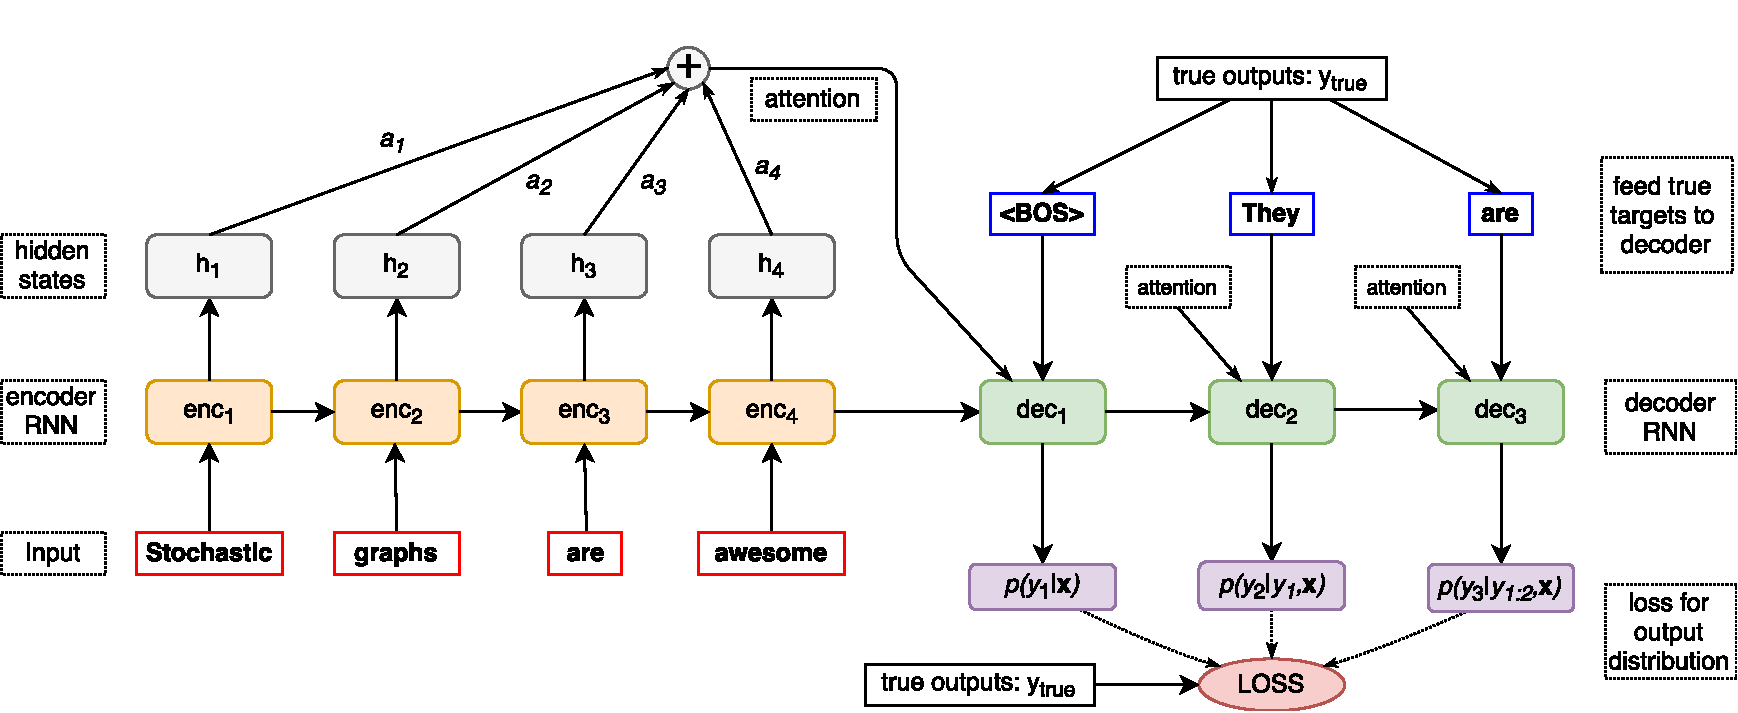
\includegraphics[width=1.0\linewidth]{seq2seq.pdf}
\caption{Пример модели seq2seq с механизмом внимания; фаза обучения}
\label{fig:seq2seq}
\end{figure}
Sequence-to-sequence модели (seq2seq \cite{seq2seq}) - это широкий класс моделей, которые предсказывают выходную последовательность из
некоторой входной последовательности. Такая архитектура применяется во многих задачах обработки естественного языка,
например таких, как машинный перевод \cite{mt} и суммаризация \cite{first_summ}.

На рисунке~\ref{fig:seq2seq} показан типичный пример seq2seq модели, состоящей из кодировщика(encoder), задача которого получить
 внутреннее представление входной последовательности, и декодера(decoder), задача которого по этому представлению получить желаемую выходную последовательность.
 В данном примере в качестве входной последовательности на вход кодировщику подается последовательность ``Stochastic graphs are awesome''.
 Кодировщих последовательно считывает последовательность, получая на каждом шаге скрытое представление $h_i$. 

 Декодер имеет внутреннее состояние, которое инициализируется представлением последовательности(последним скрытым состоянием), полученным из кодировщика.
Далее декодер на каждом шаге предсказывает условное распределение на текущий элемент последовательности при условии входной последовательности и предыдущих элементов последовательности. 
При подходе teacher forcing \cite{teacher_forcing} в качестве предыдущих элементов последовательности берутся слова из целевого предложения.
Это обеспечивается тем, что на каждом шаге декодер получает на вход предыдущее слово из целевого предложения.
На рисунке~\ref{fig:seq2seq} также показано как во время начала декодирования декодер получает на вход слово, обозначающее начало предложения -- <BOS>.
Помимо слова из целевого предложения декодер получает ``контекстный вектор'', полученный с помощью механизма внимания, который будет описан ниже в разделе \ref{attention_mechasm}.

Одним из подходов к тренировке таких моделей является максимизация правдоподобия истинной последовательности при условии входной последовательности и предыдущих
истинных элементов последовательности. Такой подход известен как teacher forcing \cite{teacher_forcing}. Несмотря на то, что метод достаточно
эффективен на практике, во время вывода(тестирования) модель не имеет доступа к истинным элементам последовательности и может использовать только свои собственные предсказания. 
Таким образом, работа модели во время тренировки и тестирования отличаются. Это приводит к двум главным проблемам:
\begin{itemize}
  \item Exposure bias \cite{Ranzato} - модель не использует свои собственные предсказания во время тренировки 
  \item Loss-evaluation mismatch \cite{Wiseman} - во время тренировки мы оптимизируем дифференцируемую метрику, но
  меряем качество другой метрикой. 
\end{itemize}

\subsubsection{Лучевой поиск в sequence-to-sequence модели}
Лучевой поиск (beam search) - это эвристический жадный алгоритм поиска пути в графе. По своей сути
он модифицирует поиск по наилучшему совпадению.
Для каждого состояния вводится функция оценки.
Во время работы алгоритма поддерживается множество лучших состояний с точки зрения функции оценки. Каждый шаг алгоритма представляет собой несколько этапов:
\begin{itemize}
  \item Сделать шаг из множества лучших состояний.
  \item Оставить только уникальные состояния, удалив лишние состояния-дубликаты.
  \item Посчитать функцию оценки для текущих состояний и выбрать по ней $beamsize$ лучших.
\end{itemize}
В задаче генерации текста алгоритм может быть применен к графу, вершинами которого являются слова, а веса ребер из каждой вершины задаются условным распределением на словах(вероятность сгенерировать слово при условии предыдущих).
Каждому состоянию будет соответствовать последовательность слов.
Оценкой для состояния будет сумма логарифмов вероятностей слов выданных декодером.
Алгоритм продемонстрирован на рисунке ~\ref{fig:beam_search} (в данном примере $beamsize=2$).

\begin{figure}[h]
\centering
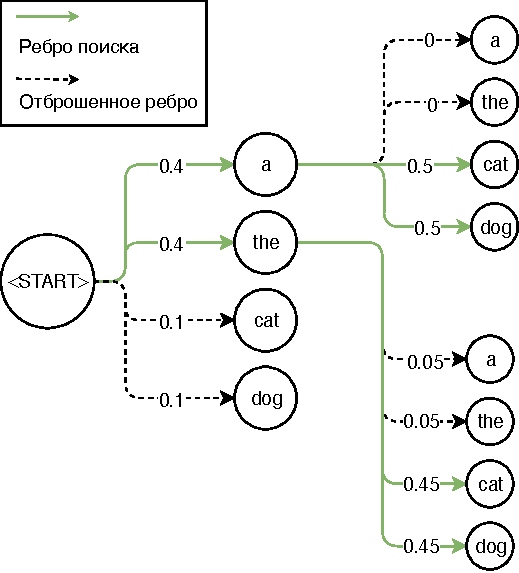
\includegraphics[width=0.5\linewidth]{beam_search.pdf}
\caption{Пример лучевого поиска осуществляемого декодером. Числа на ребрах - это вероятности сгенерировать слово.}
\label{fig:beam_search}
\end{figure}

\subsubsection{Механизм внимания в sequence-to-sequence модели}
\label{attention_mechasm}
Проблема seq2seq моделей(без механизма внимания) в том, что кодировщик должен представить всю входную последовательность
в виде вектора конечной размерности.
Механизм внимания или просто внимание -- это метод, который часто используется в seq2seq моделях для решения этой проблемы.
Он может быть использован для того, чтобы во время декодирования обращаться напрямую к:
\begin{enumerate}
  \item Состояниям кодировщика.
  \item Предыдущим состояниям декодера.
\end{enumerate}
В данной работе используется первый вариант.
Используя внимание можно получить так называемый контекстный вектор как взвешенное среднее скрытых состояний кодировщика $e_1 ... e_m$
$$ c_i = \sum\limits_j a_{i, j} e_j $$
$$ a_i = softmax(f_{att}(h_i, e_j)) $$
Алгоритм продемонстрирован на рисунке \ref{fig:attention}.
Функция $f_{att}(h_i, e_j)$ вычисляет выравнивание(alignment) между скрытым состояниями $h_i$ и $e_j$
В работе используется мультипликативное внимание.
При таком подходе $f_{att}$ вычисляется как:
$$ f_{att} = h_i^T W_a e_j  $$
$W_a$ -- это обучаемые параметры внимания.

\begin{figure}[h]
\centering
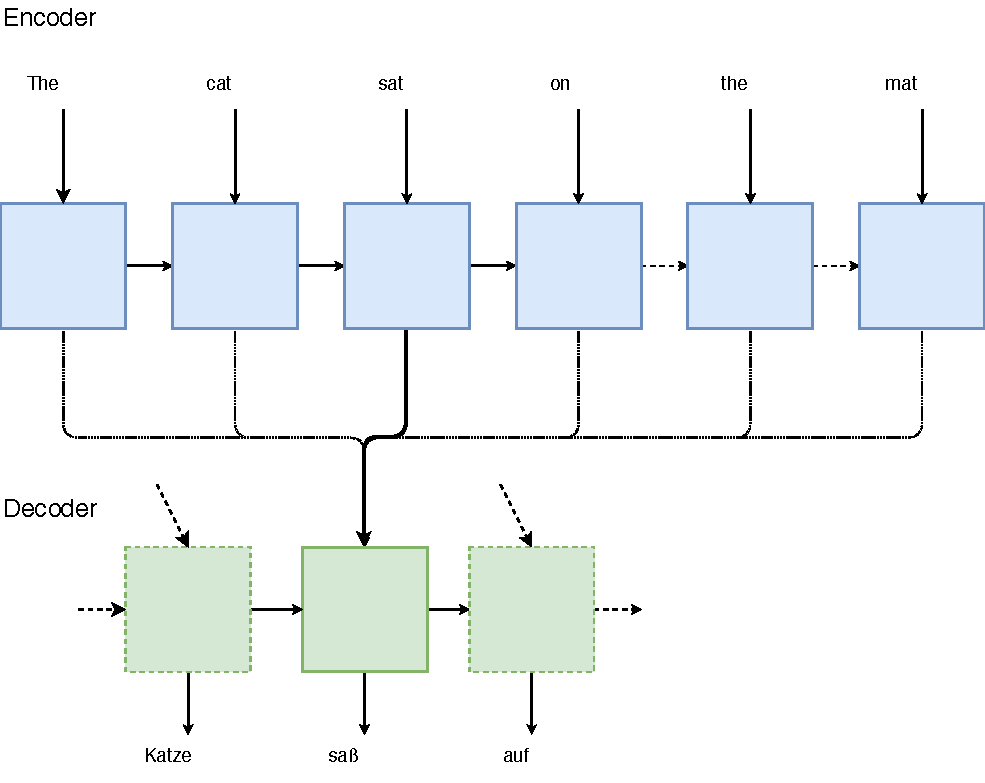
\includegraphics[width=0.7\linewidth]{attention.pdf}
\caption{Иллюстрация обученного механизма внимания. Во время генерации слова ``saß'', с большим весом берется состояние
 кодировщика соответствующего моменту времени, когда на вход подавалось слово ``sat''.}
\label{fig:attention}
\end{figure}


\subsection{Обучение с подкреплением и правило REINFORCE}
Несмотря на то, что терминология обучения с подкреплением в задаче оптимизации недифференцируемой метрики не является необходимой \cite{Minimum_Risk},
приведем здесь описание правила REINFORCE именно в этих терминах.

\begin{figure}[h]
\centering
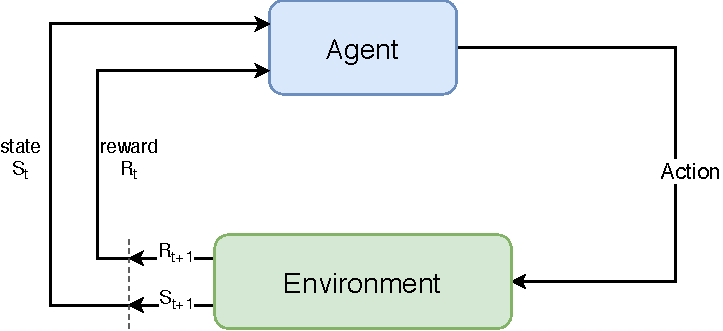
\includegraphics[width=0.5\linewidth]{MDP.pdf}
\caption{Взаимодействие агента со средой в Марковском процессе принятия решений}
\label{fig:MDP}
\end{figure}


Марковский процесс принятия решений(MDP --- Markov decision process) -- это процесс в котором участвуют агент и среда.
Процесс подразумевает собой взаимодействие среды и агента. Это взаимодействие происходит последовательно и изображено на рисунке \ref{fig:MDP}.
Агент -- это некоторый алгоритм, который в каждый момент времени в ходе марковского процесса принятия решений выбирает действие. Среда в соответствующий момент времени реагирует на это действие,
и агент оказывается в новом состоянии(среда дает новое состояние агенту). Помимо состояния среда дает агенту награду -- значение, которое
пытается максимизировать агент в ходе взаимодействия со средой.

Более формально (конечный марковский процесс приятия решений):
\begin{itemize}
  \item Состояние $S_t \in \mathcal{S}$ - это представление среды в момент времени $t \in \{0, 1, 2, 3 ...\}$, полученное агентом.
  \item В момент времени $t$ агент может выбрать действие $A_t \in  \mathcal{A}$.
  \item После того как агент выбрал действие,
 он получает награду $R_t \in \mathcal{R} \subset \mathbb{R}$ и оказывается в состоянии $S_{t+1}$
\end{itemize}

Для принятия решений агенты используют так называемую политику. Политика $\pi$ -- это отображение из $\mathcal{S}$ в
распределение на возможных действиях для данного состояния. Если это распределение вырожденное для всех состояний, то такую политику называют детерминистической,
иначе стохастической.

Траектория -- это последовательность состояний и действий (иногда в траекторию также включают и  награды) $$\tau = S_0 A_0 (R_1) S_1 A_1 (R_2) ...$$
Траекторию можно задать также относительно политики $\pi$(обозначение $\tau_{\pi}$), тогда в каждый момент времени $t$ действием будет
являться случайная величина порожденная распределением $\pi_t(S_t)$.

% Given that BLEU score is non-differentiable, a common approach is to use techniques from RL, specifically REINFORCE rule \cite{reinforce} for optimization of its expectation:

Общим подходом для оптимизации недифференцируемых метрик является использование методов из обучения с подкреплением(RL -- reinforcement learning), 
например, REINFORCE, который позволяет оптимизировать
математическое ожидание нужной метрики.

$$J(\theta) = \mathbb{E}_{\tau\sim \pi_{\theta}} \lbrack R(\tau) \rbrack
$$
\begin{equation}
\Rightarrow \nabla_\theta J(\theta) = \mathbb{E}_{\tau} \lbrack \sum_t R_t \nabla_\theta\log \pi_{\theta}(a_t|s_t) \rbrack
\label{eq:reinforce_rule}
\end{equation}


Здесь $R(\tau)$ это общая награда полученная агентом во время прохождения траектории $\tau$: $R(\tau)=\sum_t R_t$. В контексте задач обработки естественного языка траектория может рассматриваться как последовательность слов сгенерированных декодером и скрытых состояний декодера $(w_1, h_1,..w_N, h_N)$, а в роли награды $R(\tau)$ может выступить метрика BLEU. Стохастическая политика $\pi_\theta(a_t|s_t)$ задается распределением на словах в момент времени $t$.
У такого подхода есть проблема -- интегрируемая случайная величина имеет довольно большую дисперсию, что делает затруднительным получение численных оценок этого интеграла.
Одним из методов борьбы с этой проблемой является подбор baseline алгоритма. Тогда вместо $R(\tau)$ используют функцию $A(\tau) = R(\tau) - R_{B}$.
Где $R_{B}$ - это награда полученная baseline алгоритмом. В RL в качестве baseline алгоритма используется value функция $V(S)$ -- математическое ожидание награды для данного состояния.

\subsection{Стохастические вычислительные графы}
\begin{figure}[h]
\centering
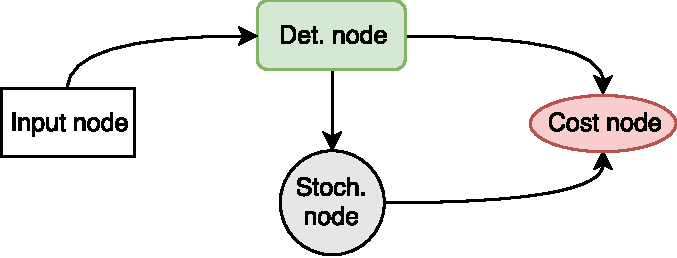
\includegraphics[width=0.5\linewidth]{scg_example.pdf}
\caption{Пример стохастического вычислительного графа}
\label{fig:scg_example}
\end{figure}
Стохастический вычислительный граф \cite{scg} - это направленный ациклический граф с тремя типами вершин:
\begin{itemize}
  \item Входные вершины
  \item Детерминистические вершины -- это функции от родительских вершин
  \item Стохастические вершины -- это распределения при условии родительских вершин.
\end{itemize}
В статье \cite{scg} доказывается следующая теорема:
\paragraph{Теорема 1.}
Примем следующие обозначения:
\begin{itemize}
  \item $\Theta$ - множество входных вершин.
  \item $\mathcal{C}$ - множество вершин ``стоимости''(cost)
  \item $\mathcal{S}$ - множество стохастических вершин.
  \item $u \prec v$ - обозначает что существует путь из $u$ в $v$.
  \item $u \prec^D v$ - обозначает что существует путь из $u$ в $v$ все вершины которого за исключением последней являются детерминистическими.
  \item $\hat{c}$ - реализация вершины ``стоимости'' $c$
  \item $\textrm{DEPS}_v = \{ w \in \Theta \cup \mathcal{S} | w \prec^D v\}.$
  
  Пусть для $\theta \in \Theta$ выполняются условия на дифференцируемость \cite{scg}, тогда
\end{itemize}
$$
  \frac{\partial}{\partial \theta} \mathbb{E}_{v \in S}\left[\sum_{c \in \mathcal{C}} c\right] =
$$
\begin{equation*}
\mathbb{E}_{v \in S}\Bigg[\underbrace{\sum_{w \in \mathcal{S}, \theta \prec^D w} \left(
\frac{\partial}{\partial \theta} \log p(w|\textrm{DEPS}_w)
\right) \sum_{c \in \mathcal{C}, w \prec c} \hat{c}}_{\textrm{(A)}}
+ \underbrace{\sum_{c \in \mathcal{C}, \theta \prec^D c} \frac{\partial}{\partial \theta}
c(\textrm{DEPS}_c)}_{\textrm{(B)}}\Bigg].
\end{equation*}
Формула состоит из двух частей:

(B) - соответствует обычному алгоритму обратного распространения ошибок.

(A) - отвечает стохастическим узлам.

Эта теорема позволяет вычислять градиенты функции ``стоимости'' по параметрам стохастического вычислительного графа.
% Каждый родитель $v$ не входной вершины $\omega$ присоединен к ней с помощью ребра $(v, \omega)$
% $$ \lrparen{asd} $$
% Now we can write down a general expression for the gradient of the expected sum of costs in a stochastic computation graph:
% $$
% \paragraph{Theorem 1.}
% \textit{Suppose that $\inp \in \cX$ satisfies \Cref{suf-cond}. Then the following two equivalent equations hold:}
% \begin{align}
% \dbyd{\inp} \Ea{
% \sum_{\outp \in \cC } \outp
% }
% &= \Ea{
% \sum_{\substack{w \in \cS,\\ \inp \precd w}}
% \left({\dbyd{\inp} \log p(w \given \anc{w} )}\right) \hat{Q}_{w}
% + \sum_{\substack{\outp \in \cC \\ \inp \precd \outp}} \dbyd{\inp} \outp(\anc{\outp})
% }
% \label{eq:mainderiv}\\
% &= \Ea{
% \sum_{\outp \in \cC} \hat{\outp}
% \sum_{\substack{w \prec \outp,\\ \theta \precd w}} \dbyd{\inp} \log p(w \given \anc{w} )
% + \sum_{\substack{\outp \in \cC,\\ \inp \precd \outp}} \dbyd{\inp} \outp(\anc{\outp})
% }.
% \label{eq:mainrearr}
% \end{align}
% $$

Вспомним две главные проблемы тренировки модели seq2seq:
\begin{itemize}
  \item Exposure bias. Модель не использует свои собственные предсказания во время тренировки.
  \item Loss-evaluation mismatch. Во время тренировки мы оптимизируем дифференцируемую метрику, но
  меряем качество другой метрикой (например BLEU)
\end{itemize}

Для того, чтобы избавиться от первой проблемы, мы могли бы подавать на вход декодеру реализацию случайной величины с распределением,
 которые он предсказал на предыдущем шаге \cite{scg_seq2seq}. Изменив таким образом модель, мы вводим случайность в процесс обучения и наш вычислительный
граф становится стохастическим (рис.~\ref{fig:train_and_inference_decoder}B).

Для решения второй проблемы можно вычислять ответы сэмплированием и распределений которые выдает декодер.


\begin{figure}
\centering
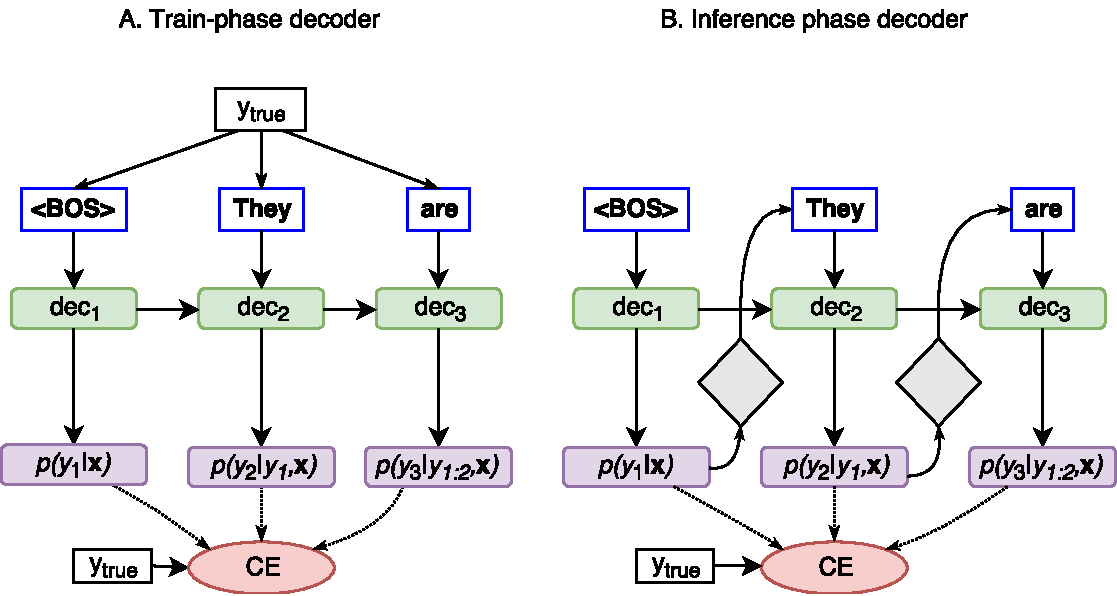
\includegraphics[width=0.9\linewidth]{train_and_inference_decoder.pdf}
\caption{Декодер во время стадий тренировки и применения}
\label{fig:train_and_inference_decoder}
\end{figure}

\section{Цель работы}
Здесь и далее будем обозначать значение метрики для конкретных предложений $x$ и $y$ как $\textrm{BLEU}(x,y)$.

Задачу максимизации математического ожидания метрики BLEU можно представить в следующем виде
\begin{equation}
\mathbb{E}_{\mathrm{data}} \mathbb{E}_{\mathrm{arch\_stoch}} \mathbb{E}_{\mathrm{output}} \textnormal{BLEU}(x, y) \to \max, 
\label{BLEU_exp}
\end{equation}
Первое математическое ожидание берется по тренировочной выборке. Второе берется по ``стохастичности сети'', которая имеет место быть если тренируемая сеть является стохастическим вычислительным графом \cite{scg}. Третье вызвано тем, что декодер предсказывает распределение на словах(элементах последовательности), а не сами слова.
В данной работе рассматривается именно третье математическое ожидание. Общим подходом для его оптимизации является формула \ref{eq:reinforce_rule}
, однако интеграл в этой формуле оказывается вычислительно трудным.
В данной работе выводится аналитическая формула дифференцируемой нижней границы метрики BLEU (BLB). Ее эффективность показывается как на
модельной задаче оптимизации, так и в задаче машинного перевода, где seq2seq модель дообученная с помощью BLB в среднем показывается лучшее качество
чем модель дообученная классическим методом REINFORCE.

\section{Постановка задачи и используемые обозначения}

\subsection{Метрика BLEU}
Метрика BLEU является одной из самых популярных метрик для оценки качества моделей генерации текста и в частности машинного перевода. Как и все подобные метрики она зависит от двух аргументов: предложения гипотезы $C$(candidate)  и истинного предложения $R$(reference). В данной работе мы не будем рассматривать метрику BLEU для корпуса и будем использовать усреднение (итоговая метрика BLEU указывается для корпуса). 
Вычисление этой метрики состоит из вычисления модифицированных точностей $p_n$ по n-граммам и штрафа за краткость BP(brevity penalty). Модифицированные точности считаются следующим образом
\begin{equation}
p_n = \frac{O_n}{\sum\limits_{C \in \{Candidates\}}^{} \sum\limits_{\textnormal{n-gram} \in C} {\textnormal{Count(n-gram)}}}
\label{p_n}
\end{equation}
Знаменатель этой дроби является ни чем иным как количеством возможных n-грамм в гипотезе $C$. Числитель состоит из так называемых ``перекрытий'' $O_n$(overlaps)
 между гипотезой $C$ и истинным предложением $R$ и рассчитывается как:
\begin{equation}
\sum\limits_{\textnormal{n-gram} \in C} \textnormal{min(Count$_C$(n-gram), Count$_R$(n-gram))}
\label{Oprime}
\end{equation}
Из формулы видно что перекрытие -- это количество общих n-грамм в C и R (суммирование ведется по различным n-граммам). 

Штраф за краткость имеет вид:
\begin{equation}
\textrm{BP} =
\begin{cases}
1 & \text{if}\ c>r \\
e^{1 - r/c} & c \le r
\end{cases}
\end{equation}

Здесь $r$ это общая длина корпуса истинных предложений, а $c$ это общая длина корпуса кандидатов. Однако в данной работе мы будем рассматривать метрику BLEU только для пары (C, R) и усреднять BLEU для пар по всему корпусу.
Таким образом BLEU считается как произведение BP и геометрического среднего точностей $p_n$ с весами $\omega_n$

\begin{equation}
\textrm{BLEU}=\textrm{BP} \cdot \exp \left(\sum\limits_{n=1}^N{w_n \log p_n}\right)
\end{equation}

Обычно $w_n = 1/N, N = 4$.


\subsubsection{Пример расчета метрики BLEU}

Проиллюстрируем приведенные обозначения на примере:

R = "Петя взял яблоко и яблоко оказалось вкусным"

C = "Яблоко"

Получаем, что $$O_1 = \min(\textrm{Count}_C(\textrm{яблоко}), \textrm{Count}_R(\textrm{яблоко})) = \min(1, 2) = 1$$
$$p_1 = \frac{1}{1} = 1, \textrm{BP} = e^{-6}$$ тогда если положить $N=1, \omega_1 = 1$ получаем
$$\textrm{BLUE} = e^{-6} \approx 0.002$$
Этот пример показывает, что несмотря на то, что точность предсказания максимально высокая, оно оказывается плохим с точки зрения метрики BLEU из-за того, что слишком короткое.
Можно сказать, что в данной метрике штраф за краткость играет роль полноты.
\section{Предлагаемый метод}
\subsection{BLEU в матричном виде}
Для вывода нижней границы необходимо переписать формулу выше в матричной форме. Рассмотрим сгенерированный текст Candidate и
истинный текст Reference и положим размер словаря равным $v$. Обозначим за
x матрицу размера $[\textrm{len}_C \times v]$, которая содержит one-hot вектора для
каждого слова в кандидате $C$. Аналогично обозначим за $y$ матрицу размера
$[\textrm{len}_R \times v]$, которая содержит one-hot вектора для каждого слова в
истинном тексте. Где $\textrm{len}_C$ и $\textrm{len}_R$ - длины Candidate и Reference текста соответственно.

Для каждой 1-граммы мы считаем матрицы  $S^{ 1}=xx^{T}$ и $P^{ 1}=yx^{T}$
размеров $\lbrack \textnormal{len$_C$} \times \textnormal{len$_C$} \rbrack$
и $ \lbrack \textnormal{len$_R$} \times \textnormal{len$_C$} \rbrack,$ соответственно:

$$
S^{ 1}_{i, j} = x_i x_j
\qquad
P^{ 1}_{i, j} = y_i x_j
$$

Аналогично определим матрицы для всех n-грамм.
\begin{equation}
S^{ n}_{i, j} = \prod\limits_{k=0}^{n-1}x_{i + k} x_{j + k}
\qquad
P^{ n}_{i, j} = \prod\limits_{k=0}^{n-1}y_{i + k} x_{j + k}
\end{equation}
Соответствующие размеры равны
$\lbrack \textnormal{len$_C$} - n + 1 \times \textnormal{len$_C$} - n + 1 \rbrack$
и $\lbrack \textnormal{len$_R$} - n + 1 \times \textnormal{len$_C$} - n + 1 \rbrack$.
Важно отметить, что элементы этих матриц обладают следующим свойством:
\begin{equation}
 S^{ n}_{i, j}=
  \begin{cases}
    1 & \text{if}\ Cand_i^n = Cand_j^n \\
    0 & \textrm{иначе}
  \end{cases}
\end{equation}
\begin{equation}
P^{ n}_{i, j}=
 \begin{cases}
   1 & \text{if}\ Ref_i^n = Cand_j^n \\
   0 & \textrm{иначе}
 \end{cases}
\end{equation}

Здесь $Cand_i^n(Ref_i^n)$ это n-грамма на позиции $i$ в предложении $C(R)$.
Для каждой n-граммы для каждой позиции в $C$ мы считаем число вхождений этой n-граммы
в $C$ или $R$.
\begin{equation}
v^{x, n}_{i} =  \sum\limits_{j=0}^{\textnormal{len$_C$} - 1} S^{n}_{j, i}
\qquad
v^{y, n}_{i} = \sum\limits_{j=0}^{\textnormal{len$_y$} - 1} P^{n}_{j, i}
\end{equation}

Наконец мы используем полученные формулы для расчета перекрытий

\begin{equation}
  O_n =
  \sum\limits_{i = 1}^{\textnormal{len}_x} \frac{\min(v^{x, n}_i, v^{y, n}_i)}{v^{x, n}_i} =
\label{o_n_2}
\end{equation}
$$ \sum\limits_{i = 1}^{\textnormal{len}_x} \min(1, \frac{v^{y, n}_i}{v^{x, n}_i}) = $$
\begin{equation}
  \sum\limits_{i = 1}^{\textnormal{len}_x} \min \Big(1,
  \frac{\sum_{j=0}^{\textnormal{len$_y$} - 1} \prod_{k=0}^{n-1}y_{i + k} x_{j + k}}{\sum_{j=0}^{\textnormal{len$_C$} - 1} \prod_{k=0}^{n-1}x_{i + k} x_{j + k}}\Big)
\end{equation}

Доказательство того, что (\ref{Oprime}) и (\ref{o_n_2}) равны, приведено в  приложении \ref{app:OO}.
Теперь мы можем посчитать модифицированные точности:
\begin{equation}
p_n = \frac{O_n}{\textnormal{len}_x - n + 1}
\label{p_n_2}
\end{equation}
Таким образом формула для рассчета метрики BLEU переписана в матричном виде и можно продолжить вывод для BLB.

Пример расчета метрики BLEU в матричном виде приведен в приложении \ref{app:matrix_bleu}

\subsection{Нижняя граница математического ожидания метрики BLEU}
Проведем вывод BLB в следующих упрощающих предположениях:

\begin{enumerate}
  \item Матрица $p_x$ размера $[\textrm{len}_C \times \textrm{vocab\_size}]$,
  которая описывает распределение на словах в последовательности $C$, детерминистически зависит от входной последовательности
  (то есть, например, отсутствует стохастичность во время декодирования).
  \item Все слова в истинной последовательности $R$ уникальны и кодируются one-hot
  векторами с помощью матрицы $y$ размера $[\textrm{len}_R \times \textrm{vocab\_size}]$
\end{enumerate}

Если мы рассмотрим стандартную seq2seq архитектуру \cite{seq2seq}, то первое предположение значит, что как только мы закодировали контекст декодер сразу детерминистически выдает матрицу вероятностей $p_x$.
Seq2seq модели во время тренировки обычно используют teacher-forcing \cite{teacher_forcing} и в этом случае первое предположение сохраняется.
Когда мы используем teacher forcing мы также игнорируем ``штраф за краткость'' (обозначается как BP), поэтому в дальнейшем выводе мы его опускаем(положим его равным 1).

Стоит отметить, что существуют более изощренные методы для тренировки seq2seq моделей, такие как например scheduled sampling \cite{scheduled_sampling}.
В этом случае вычислительный граф декодера включает в себя стохастические вершины \cite{scg_seq2seq} и генерация матрицы $p_x$ по входному тексту является случайным процессом, поэтому первое предположение не сохраняется.

%Consider somewhat simplified version of decoding task \cite{seq2seq}. Assume decoder does %not have any stochastic nodes in computational graph \cite{scg_seq2seq},
%Many standard models fall into this category, for example any sequence-to-sequence %\cite{seq2seq} model with soft attention \cite{attn} trained by teacher forcing approach %\cite{teacher_forcing}.

Обозначим за $p_y$ матрицу состоящую из one-hot векторов которые представляют последовательность $R$.
Приведем план вывода BLB:
\begin{enumerate}
  \item Записать математическое ожидание метрики BLEU используя распределение $p_x$ и вырожденное распределение $p_y$
  \item Обозначить предположения необходимые для вывода нижней оценки для интеграла.
  \item Рассмотреть случай вырожденного распределения $p_x$ (матрица состоит one-hot векторов) и показать связь выведенной оценки с обычным BLEU.
  \item Будем рассматривать значения $p_x$ как параметры функции потерь (-BLB в данном случае). Градиенты функции потерь по параметрам могут быть посчитаны с помощью программ автоматического дифференцирования \cite{pytorch}.
\end{enumerate}


Для начала напишем формулу для математического ожидания $\textrm{BLEU}(x, y)$ по распределению $p_x$ при фиксированном $y$. Оно по определению равно третьему математическому ожиданию в формуле \ref{BLEU_exp}. Обозначим его как $\textrm{BLEU}$:

\begin{equation}
\begin{split}
\textrm{BLEU} = \mathbb{E}_{\mathrm{output}} \textnormal{BLEU}(x, y) =\mathbb{E}_{x\sim p_x} \textrm{BLEU}(x, y) =\\
\mathbb{E}_{x\sim p_x} \Big \lbrack  \exp \Big(\sum_{n=1}^N \omega_n \log p_n \Big) \Big \rbrack
\label{gen_rbleu}
\end{split}
\end{equation}

BLEU это математическое ожидание произведения отдельных множителей соответствующих n-граммам. Оно может быть ограничено снизу произведением математических ожиданий.

\begin{equation}
\begin{split}
\textrm{BLEU} = \mathbb{E}_{x \sim p_x}  \Bigg \lbrack \exp\left(\sum\limits_{n=1}^N{w_n \log p_n} \right) \Bigg \rbrack \\
\geq  \prod_{n=1}^{N}  \big(\mathbb{E}_{x \sim p_x} \lbrack p_n \rbrack \big)^{\omega_n} - 1
\label{bleu_prod}
\end{split}
\end{equation}
Последняя оценка тривиальна, т.к. $p_n$ неотрицательны(и приведена лишь для строгости выкладок, однако на практике
оценка оказывается довольно близкой к реальному значению).
Рассмотрим один из множителей этого произведения. Из равенства (\ref{p_n_2})
$p_n$ с точностью до константы равен сумме перекрытий по n-граммам. Таким образом, для униграмм (BLEU1) имеем:

\begin{equation}
\begin{split}
\mathbb{E}_{x\sim p_x} \lbrack \sum_{i=1}^{len_x}{O_1^i} \rbrack =
\mathbb{E}_{x\sim p_x} \Big \lbrack \sum_{i=1}^{len_x} \frac{\min(v^{y, 1}, v^{x,1})}{v^{x, 1}} \Big \rbrack
\label{bleu_1}
\end{split}
\end{equation}

Используя неравенство Йенсена и определения $v^x, v^y$ мы можем вывести BLB для $i$-той компоненты перекрытия (приложение \ref{app:unigramLB}):

\begin{equation}
  \mathbb{E}_{x\sim p_x} \lbrack O_1^i \rbrack \geq \sum_n p_x^{in} \cdot \min \big(1, \frac{\sum_j y_{jn}}{1+\sum_{k\neq i} p_x^{kn}}\big)
\end{equation}
Таким образом нижняя оценка для компонент $O_1$ может быть вычислена используя $p_x$ и $y$. Нижняя оценка для n-грамм для $n>1$ имеет похожий вид, что и для униграмм (приложение \ref{app:n-grams}):

\begin{equation}
\begin{split}
  \label{bleu_n}
  \mathbb{E}_{x\sim p_x} \big[O_n^i \big] \geq   \sum_{m_0} p_x^{i,m_0} .. \sum_{m_{n-1}} p_x^{i+n-1,m_n} \cdot \\
 \cdot \min \big(1, \frac{\sum_j \prod_{k=0}^{n-1} y_{j + k, m_k}}{1 + \sum_{l \ne i} \prod_{k=0}^{n-1} p_x^{l+k,m_k}} \big)
\end{split}
\end{equation}
Выведенная оценка обладает важным свойством, что если $p_x$ и $p_y$ вырожденные распределения(вероятности слов либо 1 либо 0), тогда оценка совпадает с точным значением BLEU(x, y). Таким образом если мы хотим оптимизировать только один тип n-грамм (например, только 4-граммы), а не общий BLEU, мы можем использовать равенство \ref{bleu_n}.
Если мы оптимизируем обычный BLEU до порядка $n$ одновременно, мы можем использовать произведение \ref{bleu_prod} этих оценок, но для такой формулы не выполняется свойство того, что она совпадает с BLEU(x, y) для вырожденных распределений.

\section{Эксперименты и результаты}
\subsection{Модельная задача}

\begin{figure}[h]
  \centering
  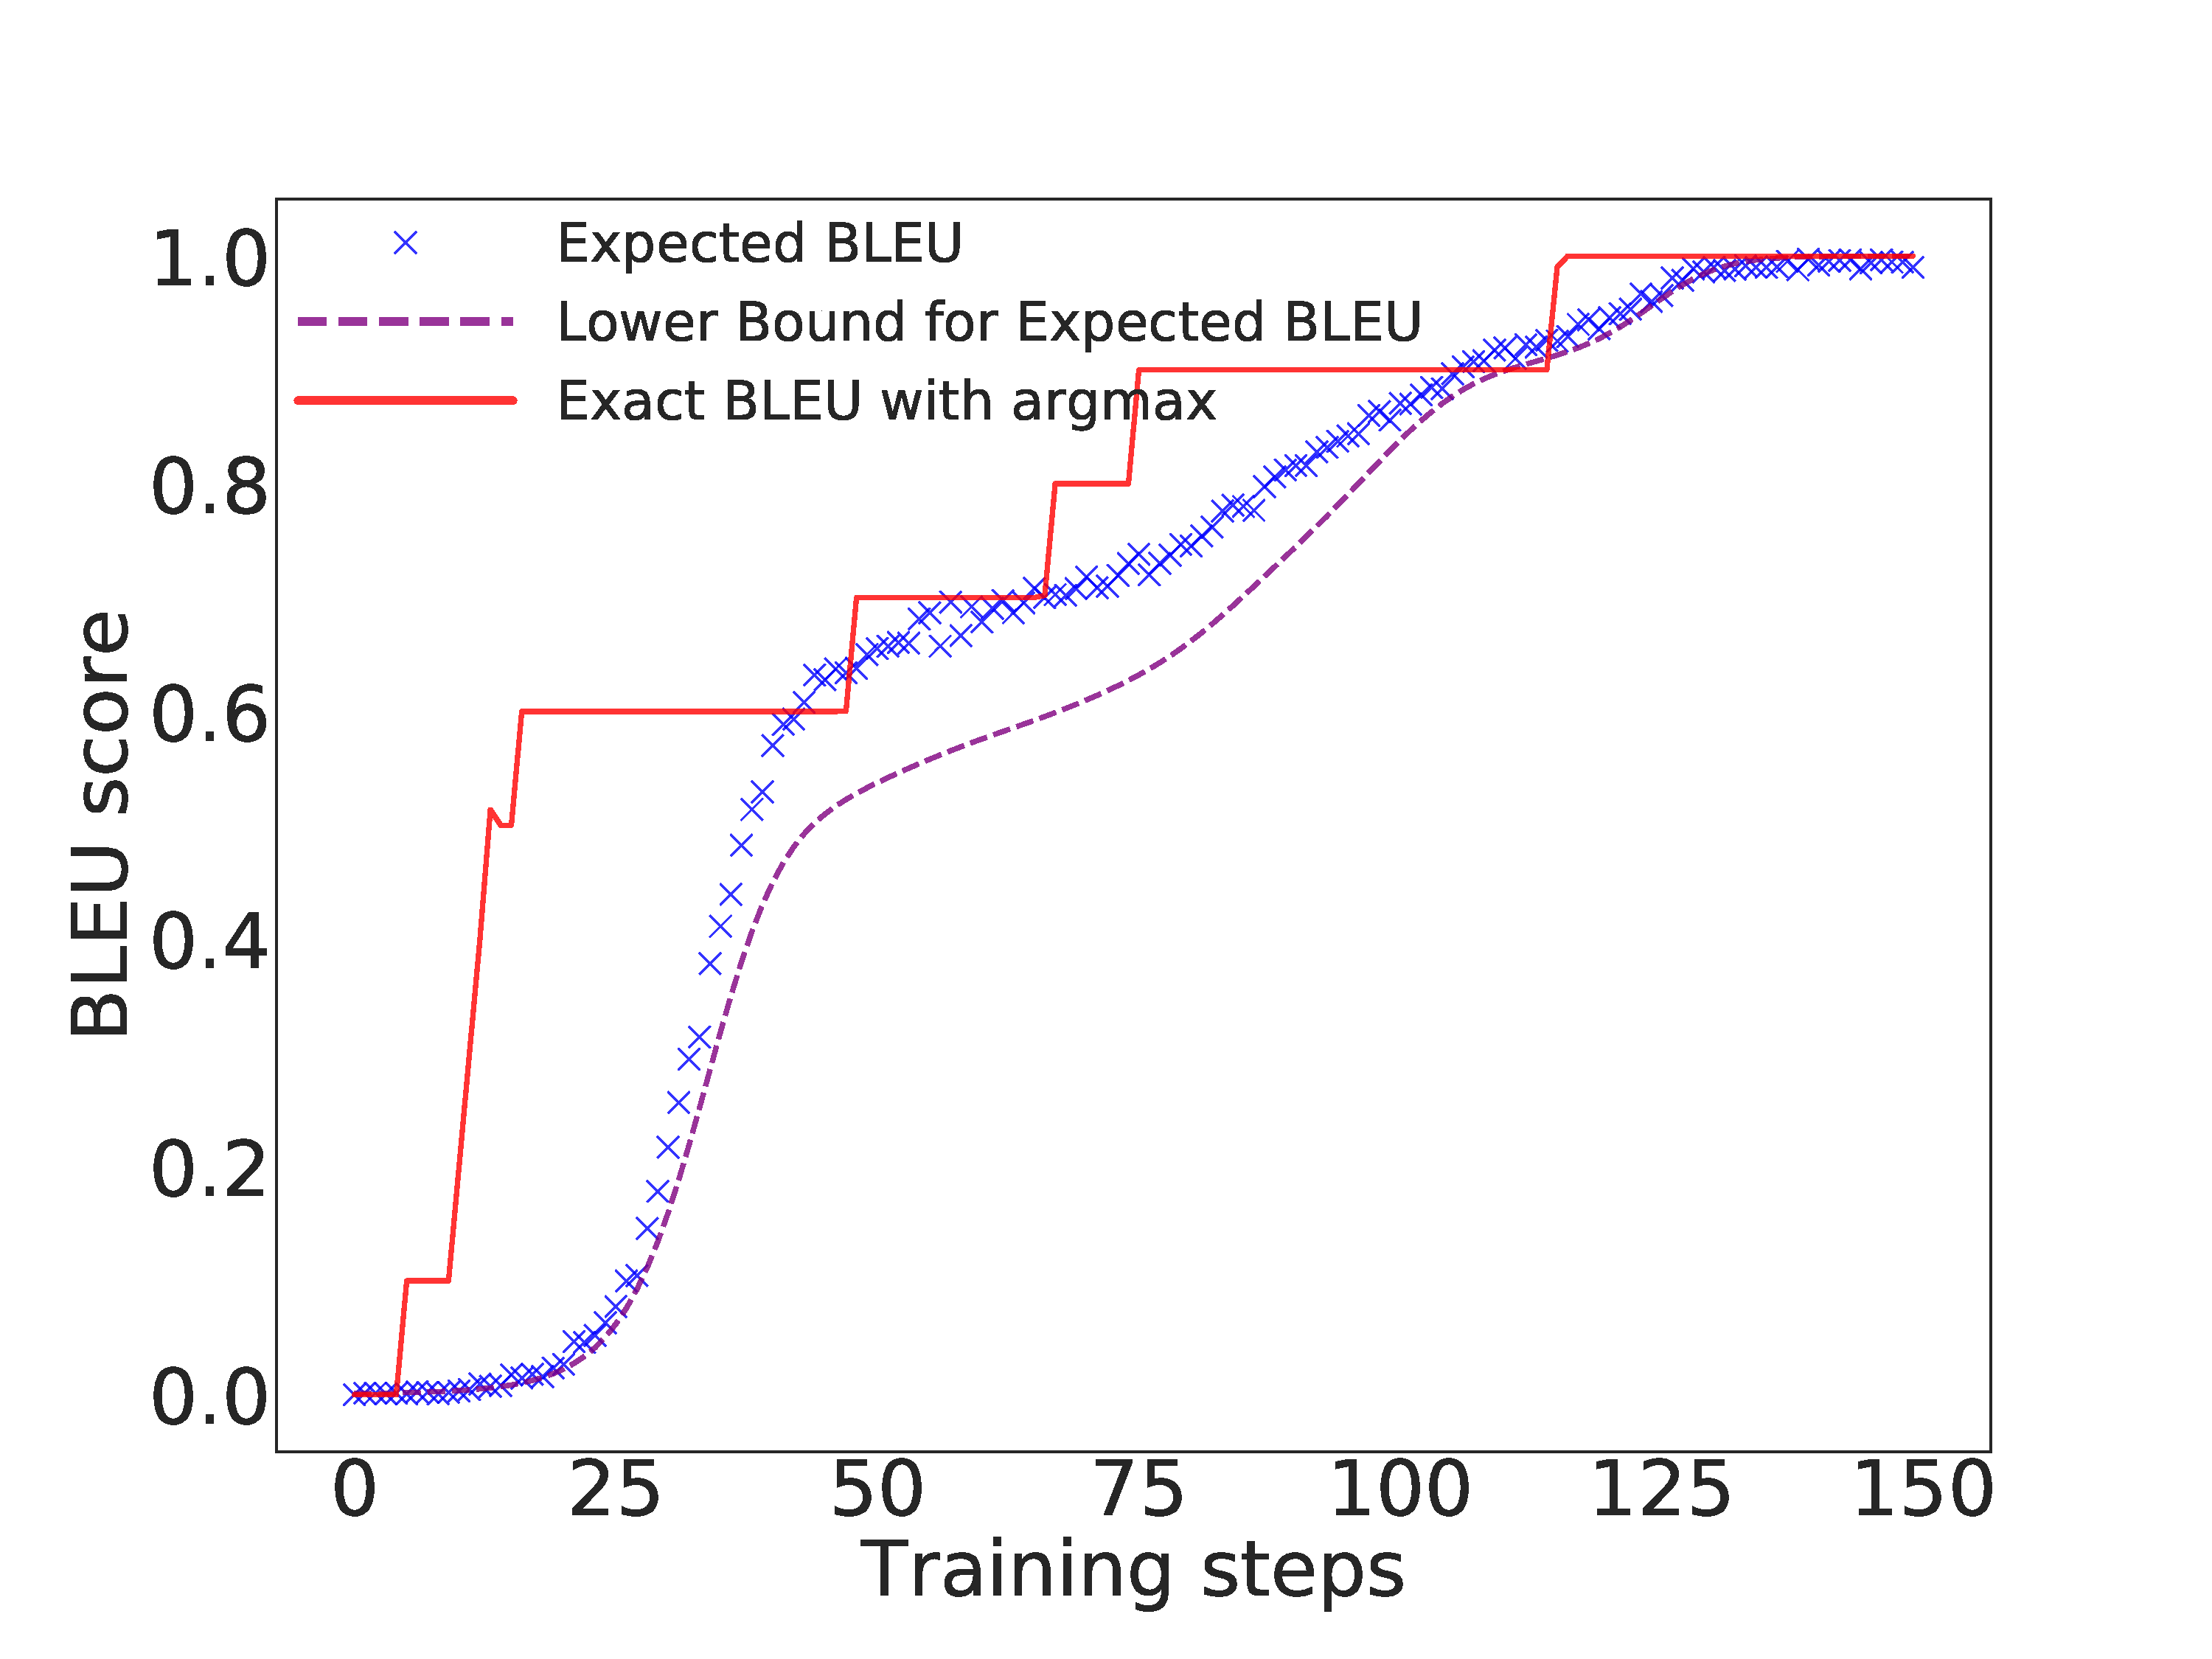
\includegraphics[scale=0.28]{BLEU_old.pdf}
  \caption{Пример кривой обучения для униграмм -- BLEU1 метрики. Красная линия -- это точный BLEU полученный применением операции $argmax$ к матрице $p_x$ построчно с последующим вычислением BLEU. Фиолетовая пунктирная линия -- это нижняя граница математического ожидания метрики BLEU (BLB). Линия из крестов обозначает математическое ожидание BLEU, полученное усреднением сэмплов из распределения $p_x$.}
  \label{fig:bleu_toy}
\end{figure}

\begin{figure}[h]
  \centering
  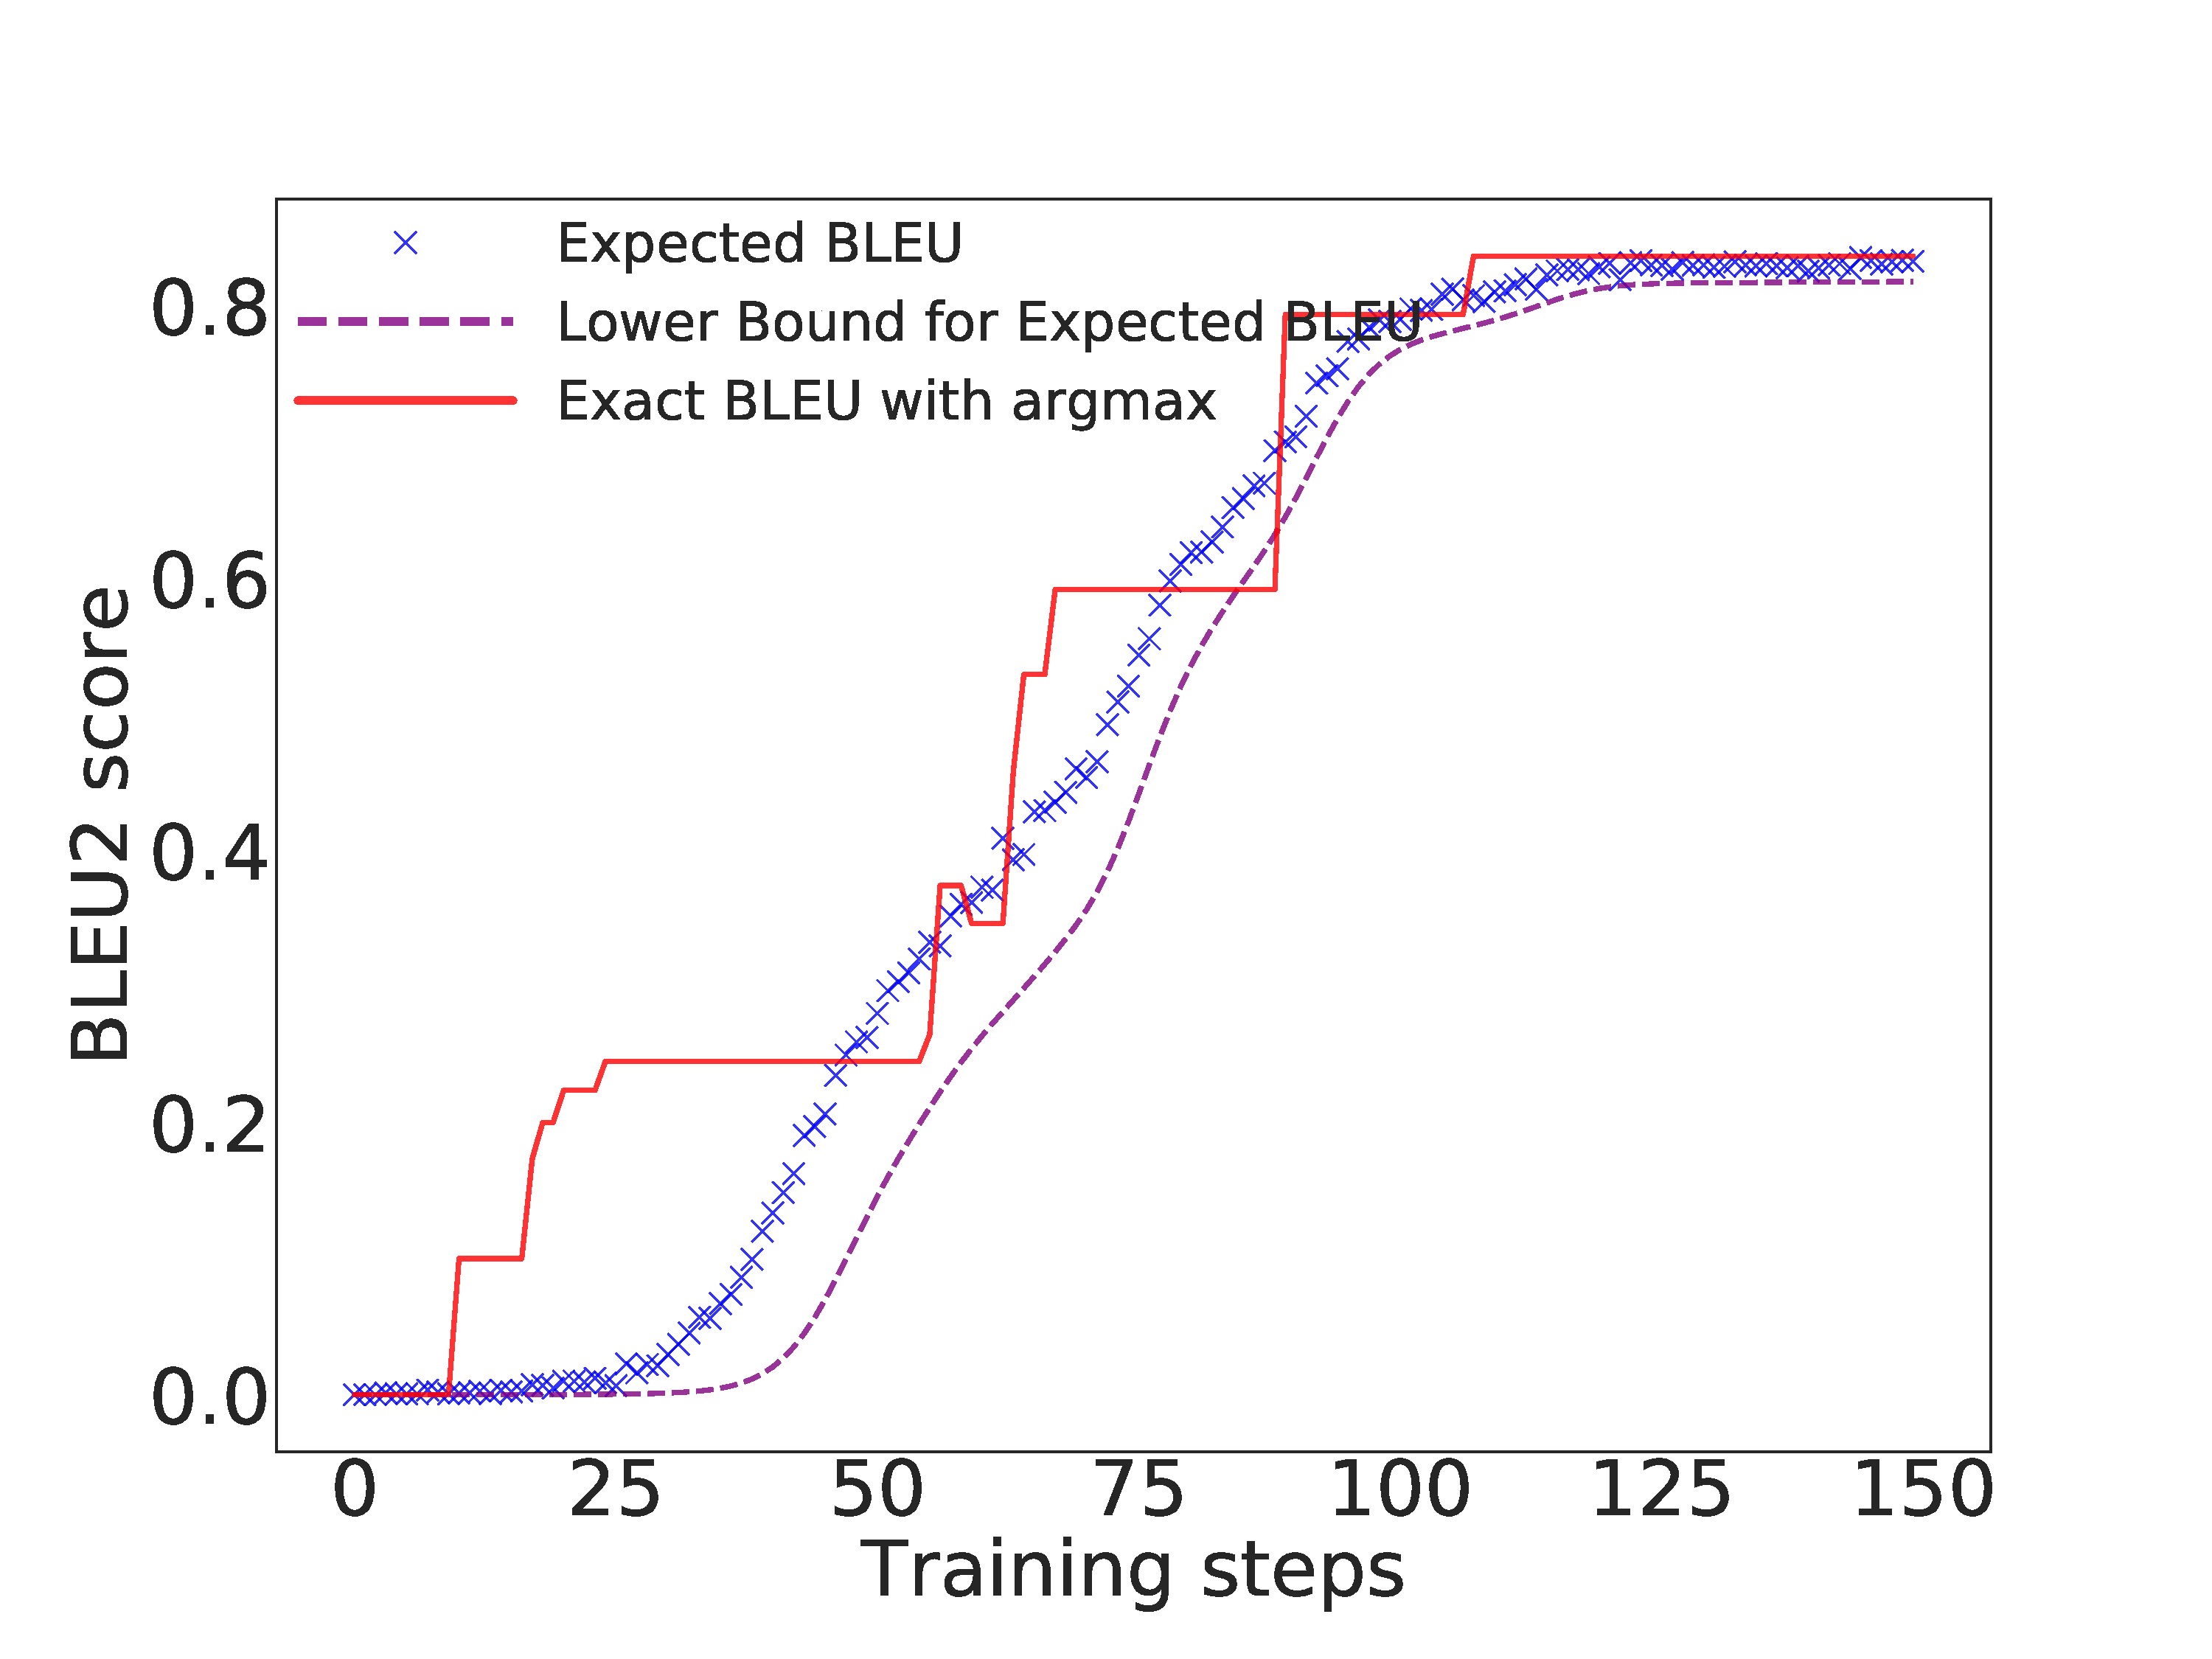
\includegraphics[scale=0.28]{BLEU2_old.pdf}
  \caption{Пример кривой обучения для биграмм (BLEU2). Линия из крестов показывает $\textrm{LB}+1$.}
  \label{fig:bleu2_toy}
\end{figure}
Для того чтобы протестировать предложенный метод был поставлен следующий эксперимент.

Генерируется матрица распределения на словах $p_x$ для перевода $C$ и матрица one-hot векторов истинного текста $r$. Обе последовательности имеют длину 10. Размер словаря выбран равным 10000.
\begin{itemize}
  \item Элементы матрицы $p_x$ сгенерированы сэмплированием значений из $\mathcal{N} (0,1)$ а затем к ним построчно применяется функция $softmax$, чтобы получить распределение вероятностей на словах.
  \item Индексы истинного текста $r$ сгенерированы сэмплированием с возвращением из равномерного распределения на множестве слов словаря.
\end{itemize}
В такой постановке нашей задачей является максимизация математического ожидания метрики BLEU между текстом сэмплированным из $p_x$ и текстом полученным из $r$. Оптимизация ведется по параметра $p_x$. Для оптимизации используется нижняя граница математического ожидания метрики BLEU.
Кривая обучения представлена на рисунке \ref{fig:bleu_toy}. График показывает скоррелированное поведение нижней оценки, точного значения метрики BLEU и его математического ожидания.

\subsection{Результаты в задаче перевода}
Мы также протестировали данный подход на датасетах для обучения машинного перевода немецко-английских пар предложений IWSLT'14 \cite{iwslt14} и англо-немецких пар WMT'14 \cite{wmt14}. Для IWSLT'14 использовалась та же предобработка текста что и в работе \cite{bso}. Для WMT'14 использовалась  предобработка предоставленная в датасете.

\begin{figure}[h]
  \centering
  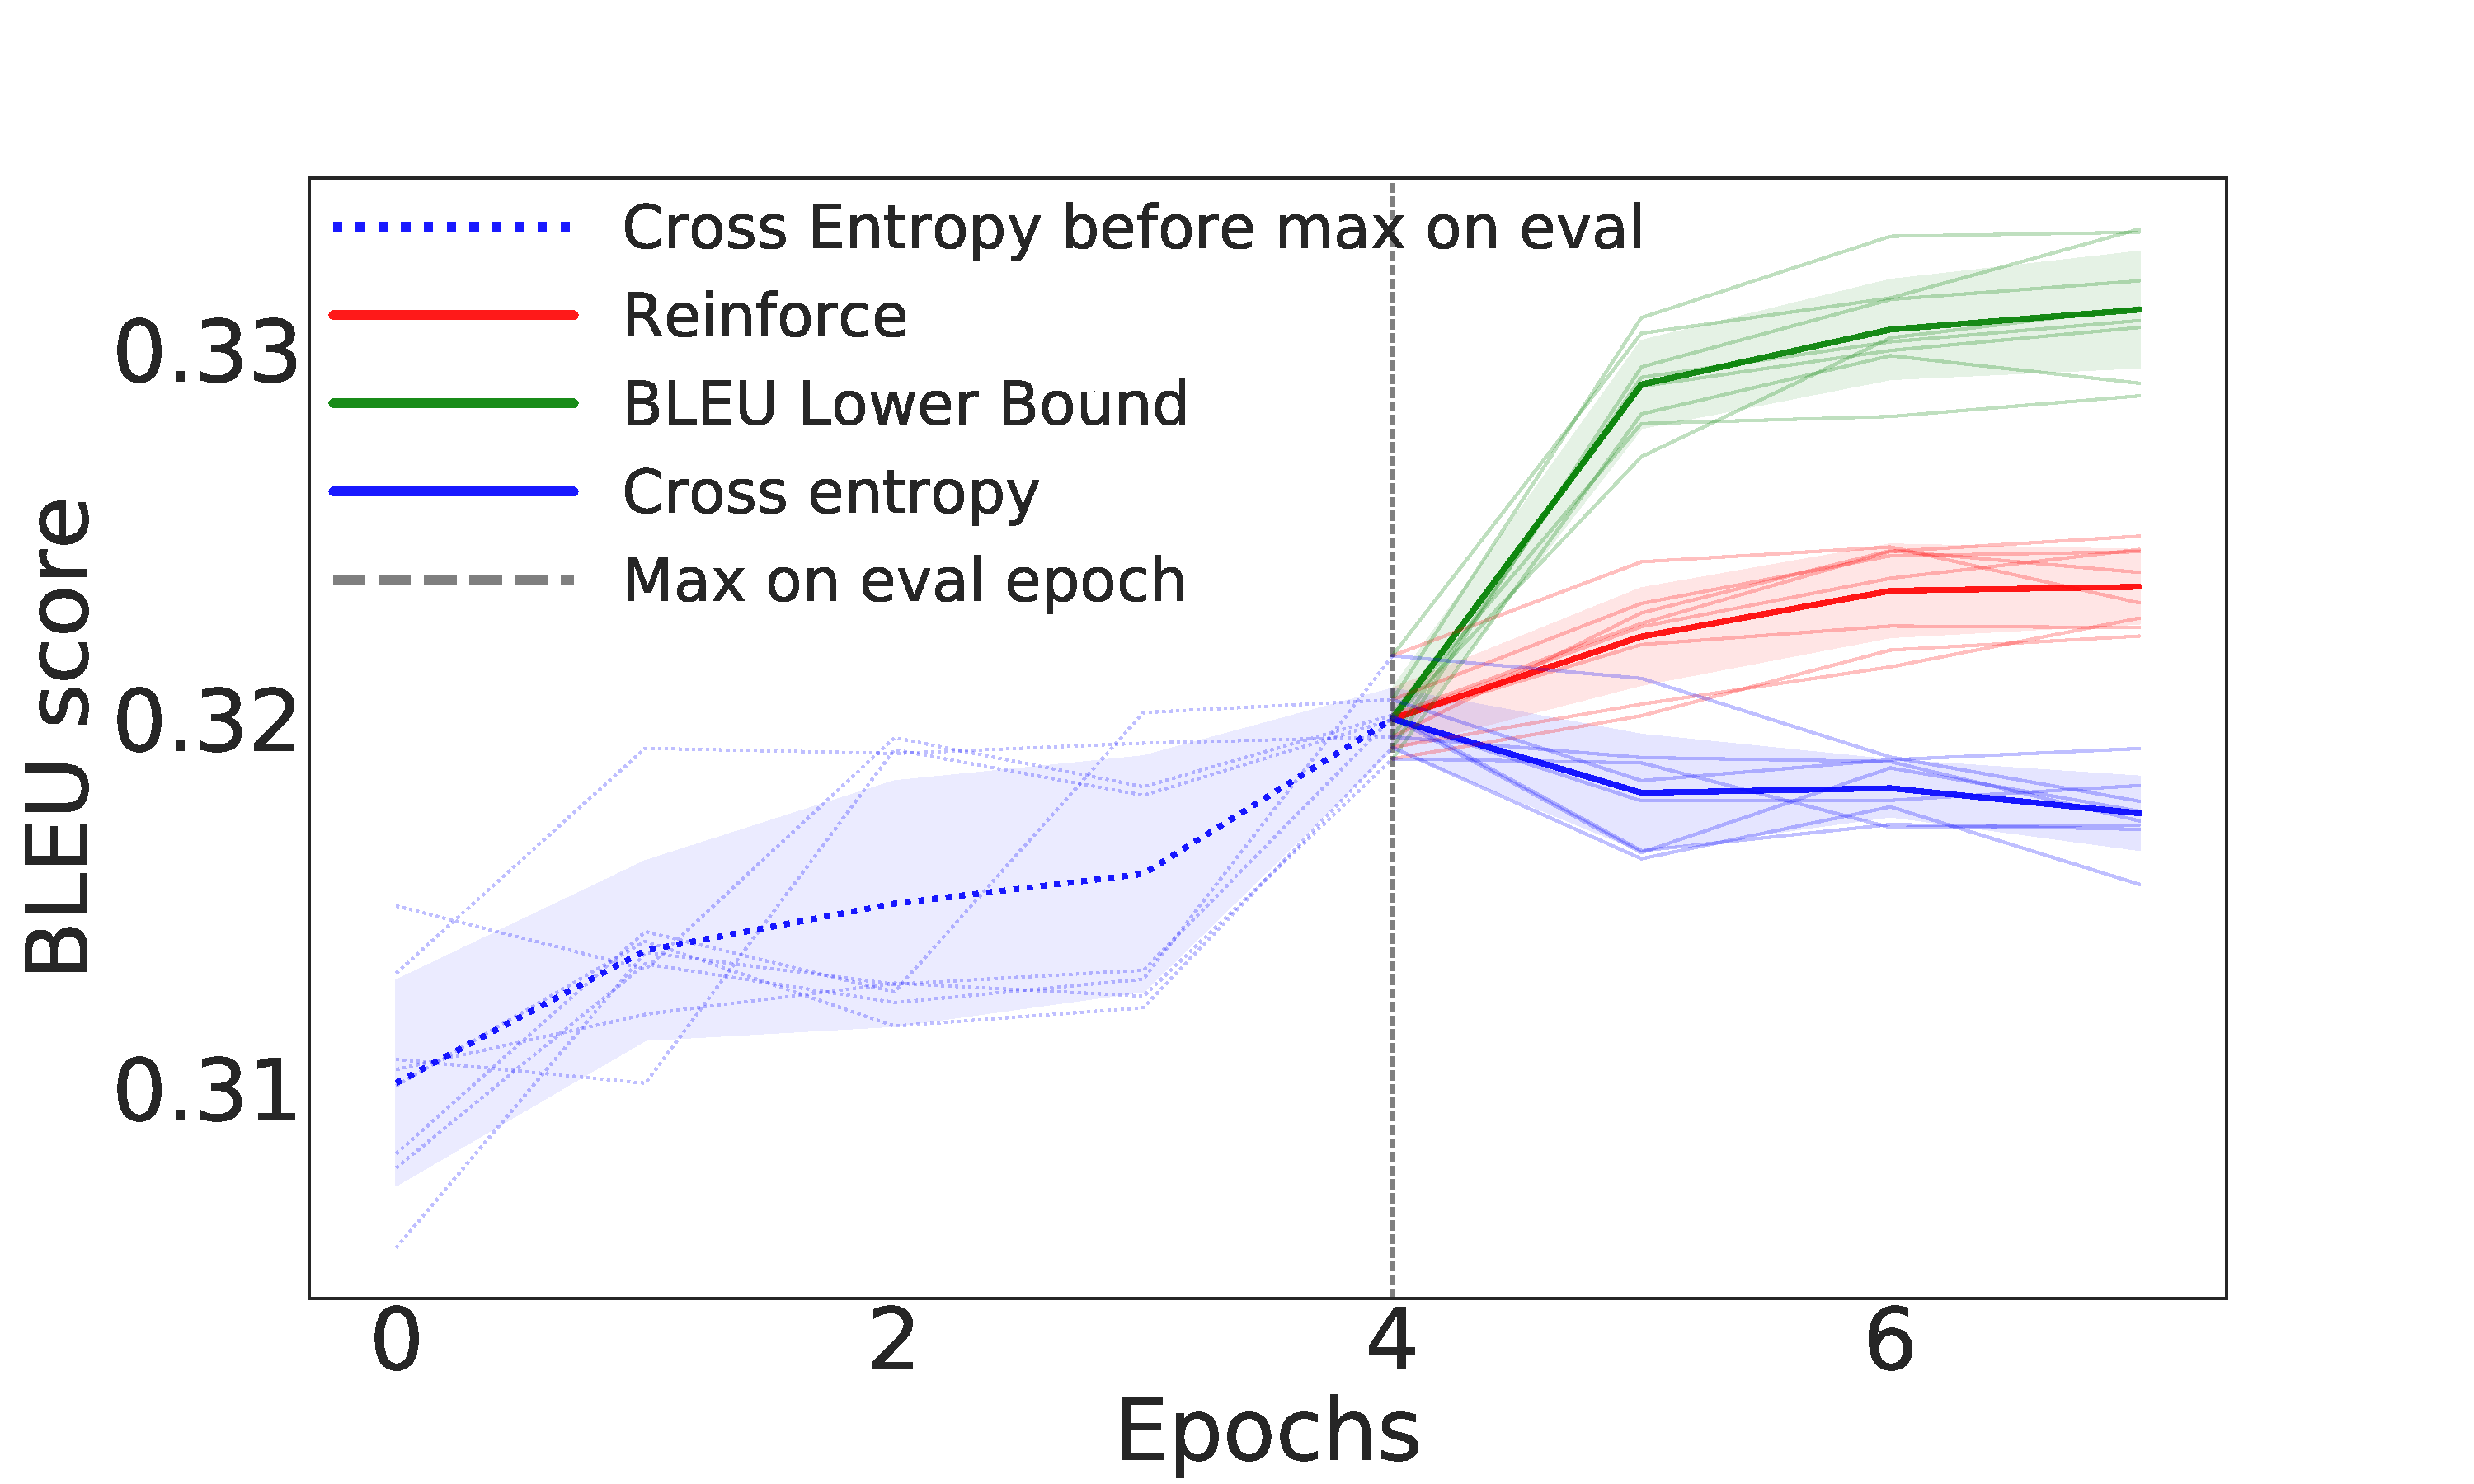
\includegraphics[scale=0.28]{res.pdf}
  \caption{Процесс обучения для разных способов оптимизации на  датасете IWSLT'14 DE$\rightarrow$EN \cite{iwslt14}. Сначала модель оптимизировалась с помощью функции потерь перекрестной энтропии. Далее, начиная с лучших весов(качество измерялось на валидационном датасете), модель оптимизировалась с помощью  перекрестной энтропии, BLB и с помощью REINFORCE. На графике указаны результаты по метрике BLEU на валидационном датасете. }
  \label{fig:results}
\end{figure}

\begin{table}[t!]
\begin{center}
\begin{tabular}{|l|ccc|}
\hline \bf & \bf CE & \bf RF & \bf LB \\ \hline
1&$26.60\pm 0.14$&$27.16\pm 0.18$&$\textbf{27.83}\pm\textbf{0.17}$\\
5&$27.56\pm 0.17$&$27.85\pm 0.11$&$\textbf{28.10}\pm\textbf{0.17}$\\
\hline
\end{tabular}
\end{center}
\caption{\label{results_translation_IWSLT} Результат на задаче перевода для датасета IWSLT'14 для трех способов оптимизации. Перекрестная энтропия (CE), REINFORCE (RF), BLEU lower bound (LB) (предлагаемый подход). Размер beamsize в лучевом поиске был равен 1 и 5. Результаты указаны по метрике BLEU на тестовом датасете.}
\end{table}

\begin{table}[t!]
  \begin{center}
  \begin{tabular}{|l|cc|}
  \hline \bf & \bf CE & \bf LB \\ \hline
  1&$17.12\pm 0.2$&$\textbf{18.65}\pm\textbf{0.13}$\\
  5&$\textbf{19.23}\pm \textbf{0.19}$&$19.03\pm 0.15$\\
  \hline
  \end{tabular}
  \end{center}
  \caption{\label{results_translation_WMT} Результат на задаче перевода для датасета WMT'14 для двух способов оптимизации. Перекрестная энтропия (CE), REINFORCE (RF), BLEU lower bound (LB) (предлагаемый подход). Размер beamsize в лучевом поиске был равен 1 и 5. Результаты указаны по метрике BLEU на тестовом датасете.}
  \end{table}
  
  

\subsubsection{Используемая модель}
Была использована стандартная seq2seq модель \cite{seq2seq}. 
Кодировщик представляет собой двунаправленный LSTM \cite{lstm} c 256 нейронами в скрытом состоянии для датасета IWSLT'14 и с 512 нейронами в скрытом состоянии для датасета WMT'14. 
Декодер представляет собой LSTM с 256 нейронами в скрытом состоянии. В декодере использовался multiplicative attention \cite{attn}, для вычисления контекстного вектора (взвешенная сумма скрытых состояний энкодера). 
Входом декодера на шаге $t$ является конкатенация представления слова на шаге $t-1$ и нелинейного преобразования контекстного вектора и скрытого состояния с предыдущего шага. 
\footnote{Имплементация доступна по ссылке \url{https://github.com/deepmipt/bleu_lower_bound}}. Во время валидации использовалось жадное декодирование и лучевой поиск с beamsize равным 1 и 5.
% Standard sequence-to-sequence framework \cite{seq2seq}was used. The encoder is bi-directional LSTM \cite{lstm} with 256 hidden units. The decoder is LSTM with 256 hidden units. In the decoder the multiplicative attention mechanism \cite{attn} was implemented for calculation of context vector (weighted hidden states of encoder). Input fed to the decoder at step $t$ is the concatenation of word embedding at step $t-1$ and non-linear transformation of context vector and hidden state of the decoder at previous step\footnote{Implementation is available at \url{github.com}}. During evaluation phase greedy decoding and beam search with beam size of 5 were tested.

\subsubsection{Детали обучения модели}
Для каждого эксперимента было сделано 8 запусков, чтобы рассчитать стандартное отклонение целевой метрики. Для оптимизации мы использовали метод оптимизации Adam \cite{adam} с learning rate равным $10^{-4}$ для  функций потерь перекрестной энтропии и BLB и $10^{-5}$ для REINFORCE.

Процесс обучения модели состоит из 4 шагов:
\begin{enumerate}
  \item Оптимизация модели с помощью перекрестной энтропии в течении 20 эпох %Optimization of model with cross-entropy loss for 20 epochs.
  \item Выбор лучших весов модели с помощью валидационного датасета. %Selecting the best model weights using results on validation set.
  \item Дальнейшая оптимизация модели(начиная с найденных весов) в течении 5 эпох с помощью одного из трех подходов: перекрестная энтропия, REINFORCE, BLB
  \item Выбор эпохи на которой модель показала лучшее качество по метрике BLEU на валидационном датасете.
\end{enumerate}
Также важно отметить, что аддитивное сглаживание (additive smoothing) для точностей в расчете метрики BLEU повышает стабильность обучения на задаче машинного перевода. 
$$\textrm{LB}\Bigg \lbrack \frac{O_n}{\textnormal{len}_x - n + 1} \Bigg \rbrack \rightarrow\frac{ \textrm{LB} \lbrack O_n \rbrack + 1}{\textnormal{len}_x - n + 2}
$$
По своей сути это стандартный трюк добавления константы под логарифм
(геометрическое среднее $p_n$ вычисляется как экспонента от суммы логарифмов), однако в экспериментах вычислительная нестабильность проявлялась только при $n > 1$.

Результаты на тестовой выборке датасета IWSLT'14 приведены в таблице ~\ref{results_translation_IWSLT} в формате ``mean $\pm$ std''. Оптимизация с помощью BLB приводит к более высоким значения метрики BLEU на тестовой выборке для обоих размеров beamsize.

Результаты на тестовой выборке датасета WMT'14 (EN-DE) приведены в таблице ~\ref{results_translation_WMT} в формате ``mean $\pm$ std''. Оптимизация с помощью BLB приводит к более высоким значениям метрики BLEU на тестовой выборке, если значение beamsize в лучевом поиске равно 1 и не приводит для beamsize равного 5. 

\section{Выводы}
Предложена вычислительно эффективная, дифференцируемая нижняя оценка для математического ожидания метрики BLEU. На задаче перевода показано, что оптимизация такой оценки ведет к повышению значения метрики BLEU в сравнении с альтернативами (cross-entropy, REINFORCE).
Для того, чтобы использовать BLB необходимы совсем незначительные изменения процесса обучения перекрестной энтропией: на последних эпохах заменить функцию потерь перекрестную энтропию на BLB. Имплементация алгоритма доступна в открытом доступе по \href{https://github.com/deepmipt/bleu_lower_bound}{ссылке}.


\newpage
% \bibliographystyle{unsrt}
\bibliographystyle{gost780}
\bibliography{main}



\newpage
\appendix
\addcontentsline{toc}{section}{Приложения}
\parttoc
\section{Пример расчета метрики BLEU в матричном виде}
\label{app:matrix_bleu}
$C="abba" \quad  R="abb"$
\renewcommand{\kbldelim}{(}% Left delimiter
\renewcommand{\kbrdelim}{)}% Right delimiter
\[
x = \kbordermatrix{
  & a & b\\
  0 & 1 & 0\\
  1 & 0 & 1\\
  2 & 0 & 1\\
  3 & 1 & 0\\
  }
\quad
y = \kbordermatrix{
  & a & b\\
  0 & 1 & 0\\
  1 & 0 & 1\\
  2 & 0 & 1\\
  }
\]
Для униграм имеем:
\[
S^1 = \kbordermatrix{
  & a & b & b & a\\
  a & 1 & 0 & 0 & 1\\
  b & 0 & 1 & 1 & 0\\
  b & 0 & 1 & 1 & 0\\
  a & 1 & 0 & 0 & 1\\
  }
\quad
P^1 = \kbordermatrix{
  & a & b & b & a\\
  a & 1 & 0 & 0 & 1\\
  b & 0 & 1 & 1 & 0\\
  b & 0 & 1 & 1 & 0\\
  }
\]

\[
v^{x, 1} = \begin{bmatrix}2 \\ 2 \\ 2 \\ 2\end{bmatrix}
\quad
v^{y, 1} = \begin{bmatrix}1 \\ 2 \\ 2 \\ 1\end{bmatrix}
\]
Для биграмм:
\[
S^2 = \kbordermatrix{
  & ab & bb & ba\\
  ab & 1 & 0 & 0\\
  bb & 0 & 1 & 0\\
  ba & 0 & 0 & 1\\
  }
\quad
P^2 = \kbordermatrix{
  & ab & bb & ba\\
  ab & 1 & 0 & 0\\
  bb & 0 & 1 & 0 \\
  }
\]

\[
v^{x, 2} = \begin{bmatrix}1 \\ 1 \\ 1\end{bmatrix}
\quad
v^{y, 2} = \begin{bmatrix}1 \\ 1 \\ 0\end{bmatrix}
\]
Для триграмм:
\[
S^3 = \kbordermatrix{
  & abb & bba\\
  abb & 1 & 0\\
  bba & 0 & 1\\
  }
\quad
P^3 = \kbordermatrix{
  & abb & bba\\
  abb & 1 & 0\\
  }
\]

\[
v^{x, 3} = \begin{bmatrix}1 \\ 1\end{bmatrix}
\quad
v^{y, 3} = \begin{bmatrix}1 \\ 0\end{bmatrix}
\]

\section{Эквивалентность формул для перекрытий $O_n$}
\label{app:OO}
Пусть $W$ обозначает множество n-грамм для $C$. $I_{\omega}$ обозначает множество начальных индексов n-грамм $\omega$ в $C$:
$$ O_n = \sum\limits_{\omega \in W} \sum\limits_{i \in I_{\omega}}
\frac{\min(v_i^{y, n}, v_i^{x, n})}{v_i^{x, n}} = (*)$$
% $$
% \left\{
%   \begin{array}{ll}
%     \forall i, j \in I_{\omega}\\
%     v_i^{x, n} = v_j^{x, n} = |I_{\omega}| = Count_C(\omega)\\
%     v_i^{y, n} = v_j^{y, n} = Count_R(\omega)
%   \end{array}
% \right\}=
%   $$
Рассмотрим n-грамму $\omega$ и $i$ - индекс где n-грамма $\omega$ начинается в переведенном предложении. Вспомним, что $v_i^{x, n}$ (и $v_i^{y, n}$) обозначают число вхождений n-граммы $\omega$ в предложение перевода.
Рассмотрим $i, j \in I_{\omega}$, тогда по определению $$v_i^{x, n} = v_j^{x, n} = Count_C(\omega) = |I_\omega|$$
$$ v_i^{y, n} = v_j^{y, n} = Count_R(\omega)$$
  $$
(*) =\sum\limits_{\omega \in W} \sum_{i \in I_{\omega}} \frac{min(Count_R(\omega), Count_C(\omega))}{Count_C(\omega)} =
  $$

  $$
  =\sum\limits_{\omega \in W} min(Count_R(\omega), Count_C(\omega))
$$
\subsection{Пример}
Рассмотрим гипотезу
$$ C = \textnormal{“Mike took an apple and the apple was delicious”}$$
Проведем пример для случая униграмм $n=1$.
Рассмотрим слово $\omega=\textnormal{apple}$, тогда $I_w = \{3, 6\}$ - начальный индексы слова apple в данном предложении.
Количество вхождений слова $\omega$ в предложение равно $$2 = |I_w| = Count_C(w)=$$  $$=v_3^{x, 1} = v_6^{x, 1}$$ по определению v.


\section{Нижняя граница для униграмм}
\label{app:unigramLB}
Вывод нижней границы для униграммной метрики BLEU:
\begin{equation}
\mathbb{E}_{x\sim p_x,y \sim p_y} O_1^i = \mathbb{E}_{x\sim p_x,y \sim p_y} \Big \lbrack \min \big(1, \frac{\sum_j x_i y_j}{\sum_k x_i x_k}\big) \Big \rbrack
\label{bleu_i_1}
\end{equation}

Разбиваем математическое ожидание на два интеграла, один из них по случайной переменной $x_i$ а оставшийся по всем остальным. Распределение на  $y$ опущено здесь и далее:

$$
= \mathbb{E}_{x_{k,k\neq i}} \Big \lbrack \sum_n p_x^{in} \min \big(1, \frac{\sum_j y_{jn}}{\sum_k x_i x_k}\big) \Big \rbrack
$$
\begin{equation}
= \sum_n p_x^{in} \cdot \mathbb{E}_{x_{k,k\neq i}} \Big \lbrack \min \big(1, \frac{\sum_j y_{jn}}{1+\sum_{k\neq i} x_i x_k}\big) \Big \rbrack
\label{bleu_i_2}
\end{equation}

Выражение в квадратных скобках может рассматриваться как функция от переменной $x_k$ на $[0,1]^n$. Эта функция является вогнутой (приложение \ref{app:convex}), поэтому мы можем применить неравенство Йенсена чтобы вывести нижнюю границу:


$$
= \sum_n p_x^{in} \cdot \mathbb{E}_{x_{k,k\neq i}} \Big \lbrack \min \big(1, \frac{\sum_j y_{jn}}{1+\sum_{k\neq i} x_i x_k}\big) \Big \rbrack
$$
\begin{equation}
\geq \sum_n p_x^{in} \cdot \min \big(1, \frac{\sum_j y_{jn}}{1+\sum_{k\neq i} p_x^{kn}}\big)
\label{bleu_i_3}
\end{equation}


\section{Обобщение для n-грамм}
\label{app:n-grams}
Запишем явно математическое ожидание по случайным величинам $\{x_{i + p}: p \in \{0..n-1\}\}$ для $i$-ой компоненты перекрытия $O_n$
% Write down explicitly mathematical expectation over random variables $\{x_{i + p}: p \in \{0..n-1\}\}$ for $i$-th component of overlap $O_n$:
$$
\mathscr{L}_i = {x_{k,k \not\in \{i + p: p \in \{0..n-1\} \} }}
$$

$$
\mathbb{E}_{x\sim p_x} \big[ O_n^i \big] =
$$
\begin{equation}
\begin{split}
\mathbb{E}_{\mathscr{L}_i}
 \Big \lbrack
\sum_{m_0} p_x^{i,m_0} ... \sum_{m_{n-1}} p_x^{i+n-1,m_{n-1}}  O_n^i
 \Big \rbrack
\label{bleu_i_2}
\end{split}
\end{equation}

Пусть $s$ это некоторый индекс и  $s \not\in \{i + p: p \in \{0..n-1\} \}$:
Рассмотрим два множества $A_{s, i} = \{l: l \ne i, s \in [l..l+n-1]\}$ и
 $B_{s, i}=\{l: l \ne i, s \not\in [l..l+n-1] \}$
и перепишем
$$O_n^i = $$
$$
\min(1, \frac{\sum_j \prod\limits_{k=0}^{n-1}y_{k + k, m_k}}
                               {1 + \sum\limits_{A_{s, i}} \prod\limits_{k=0}^{n-1} x_{i + k}x_{l + k}
                                  + \sum\limits_{B_{s, i}} \prod\limits_{k=0}^{n-1} x_{i + k}x_{l + k}})$$
Поменяем порядок интегрирования и запишем отдельно математическое ожидание по $p_x^s$,
\begin{equation}
\begin{split}
\sum_{m_0} p_x^{i,m_0} ... \sum_{m_{n-1}} p_x^{i+n-1,m_n} \\
\mathbb{E}_{x_{k,k \not\in \{i + p: p \in \{0..n-1\} \}, k \ne s} } \mathbb{E}_{p_x^s} O_n^i
\label{bleu_i_3}
\end{split}
\end{equation}


Математическое ожидание по случайной величине $x^s$ имеет следующий вид:

$$ \min(1, \frac{A}{1 + B + \vec{c} x_s})$$

Где $A, B$ некоторые константы и $\vec{c}$ константный вектор:

$$\frac{A}{1 + B + \vec{c} x_s}$$

Поскольку это выпуклая функция (приложение \ref{app:convex}), мы можем применить неравенство Йенсена последовательно для всех $s \not\in \{i + p: p \in \{0..n-1\} \}$.

Новыми $O_n^i$ будут $$O_i^{'n}=\min \big(1, \frac{\sum_j \prod_{k=0}^{n-1} y_{j + k, m_k}}{1 + \sum_{l \ne i} \prod_{k=0}^{n-1} p_x^{l+k,m_k}} \big)$$
Итоговое неравенство:
$$\mathbb{E}_{x\sim p_x} \big[O_n^i \big]  \geq \sum_{m_0} p_x^{i,m_0} .. \sum_{m_{n-1}} p_x^{i+n-1,m_n} O_i^{'n}
\label{bleu_i_4}$$

\section{Доказательство выпуклости}
\label{app:convex}
Обозначим за $a$ фиксированный вектор, а $A, B$ некоторые положительные константы:
\begin{equation}
\frac{A}{B + a((1 - \alpha)x_s + \alpha y_s)}
\le \frac{(1 - \alpha)A}{B + a x_s} + \frac{\alpha A}{B + a y_s}
\end{equation}
Без ограничения общности:
\begin{equation}
\frac{1}{1 + a((1 - \alpha)x_s + \alpha y_s)}
\le \frac{1 - \alpha}{1 + a x_s} + \frac{\alpha}{1 + a y_s}
\end{equation}

Обозначим $S = a x_s$, $T = a y_s$:

$$
\frac{1}{1 + (1 - \alpha)S + \alpha T} \le \frac{1 - \alpha}{1 + S} + \frac{\alpha}{1 + T}
$$

$$
\frac{1}{1 + (1 - \alpha)S + \alpha T} \le
\frac{(1 - \alpha)(1 + T) + \alpha (1 + S)}{(1 + T)(1 + S)}
$$
$$
\frac{1}{1 +  (1 - \alpha)S + \alpha T} \le
\frac{1 + (1 - \alpha)T + \alpha S}{(1 + T)(1 + S)}
$$
$$
\ln(1 + T) + \ln(1 + S) \le
$$
$$
\ln(1 + (1 - \alpha)S + \alpha T) + \ln(1 + (1 - \alpha)T + \alpha S)
$$

Поскольку функция $\ln(1 + x)$ выпуклая:

$$
\ln(1 + (1 - \alpha)S + \alpha T) \ge$$
$$
(1 - \alpha)\ln(1 + S) + \alpha \ln(1 + T)
$$
$$
\ln(1 + (1 - \alpha)T + \alpha S) \ge (1 - \alpha)\ln(1 + T) + \alpha \ln(1 + S)
$$

\section{Полные результаты экспериментов на датасете IWSLT}
\begin{table}[!htbp]
\begin{tabular}{| l  c |}
\hline \bf LB & \bf CE\\
\hline
\bf 28,16 & 26,67\\
\bf 27,73 & 26,73\\
\bf 27,65 & 26,42\\
\bf 28,08 & 26,73\\
\bf 27,88 & 26,70\\
\bf 27,95 & 26,36\\
\bf 27,7  & 26,64\\
\bf 27,85 & 26,57\\
\hline
\end{tabular}
\quad \quad \quad \quad \quad \quad \quad \quad \quad \quad \quad
\begin{tabular}{| l  c |}
  \hline \bf LB & \bf CE\\
  \hline
  $\textbf{27,87}\pm \textbf{0,18}$ & $26,60\pm 0,14$\\
  \hline
  \end{tabular}
  \caption{Результаты по метрике BLEU для двух способов оптимизации: Перекрестная энтропия (CE), BLEU lower bound (LB).
           В таблице слева результаты приведены для восьми экспериментов с разной начальной инициализацией(для различных значений random seed).
           В таблице справа указаны агрегированные результаты в формате ``mean $\pm$ std''.\\
           Значения получены для лучевого поиска с beamsize=1 (жадное декодирование).}
\end{table}
\begin{table}[!htbp]
\begin{tabular}{|l  c  | r|}
  \hline
  \bf LB & \bf CE\\
  \hline
  \bf 28,33 & 27,72 \\
  \bf 28,05 & 27,77 \\
  \bf 27,84 & 27,27 \\
  \bf 28,32 & 27,63 \\
  \bf 28,11 & 27,65 \\
  \bf 28,18 & 27,52 \\
  \bf 27,93 & 27,51 \\
  \bf 28,06 & 27,41 \\
  \hline
\end{tabular}
\quad \quad \quad \quad \quad \quad \quad \quad \quad \quad \quad
\begin{tabular}{| l  c |}
  \hline
  \bf LB & \bf CE\\
  \hline
  $\textbf{28,10}\pm \textbf{0,17}$ & $27,56 \pm 0,16$ \\
  \hline
\end{tabular}
\caption{Результаты по метрике BLEU для двух способов оптимизации: Перекрестная энтропия (CE), BLEU lower bound (LB).
В таблице слева результаты приведены для восьми экспериментов с разной начальной инициализацией(для различных значений random seed).
В таблице справа указаны агрегированные результаты в формате ``mean $\pm$ std''.\\
Значения получены для лучевого поиска с beamsize=5.}
\end{table}

\begin{table}[!htbp]
\begin{tabular}{|l  c |}
  \hline
  \bf RF & \bf CE\\
  \hline
  \bf 27,42 & 26,67\\
  \bf 27,09 & 26,73\\
  \bf 27,03 & 26,42\\
  \bf 27,15 & 26,73\\
  \bf 27,29 & 26,70\\
  \bf 26,82 & 26,36\\
  \bf 27,19 & 26,64\\
  \bf 27,27 & 26,57\\
  \hline
\end{tabular}
\quad \quad \quad \quad \quad \quad \quad \quad \quad \quad \quad
\begin{tabular}{| l  c |}
  \hline
  \bf RF & \bf CE\\
  \hline
   $\textbf{27,16}\pm \textbf{0,18}$ & $26,60\pm 0,14$ \\
   \hline
\end{tabular}
\caption{Результаты по метрике BLEU для двух способов оптимизации: Перекрестная энтропия (CE), правило REINFORCE (RF).
В таблице слева результаты приведены для восьми экспериментов с разной начальной инициализацией(для различных значений random seed).
В таблице справа указаны агрегированные результаты в формате ``mean $\pm$ std''.\\
Значения получены для лучевого поиска с beamsize=1 (жадное декодирование).}
\end{table}

\begin{table}[!htbp]
\begin{tabular}{|l  c |}
  \hline
  \bf RF & \bf CE \\
  \hline
  \bf 28,06 & 27,72 \\
  \bf 27,9  & 27,77 \\
  \bf 27,66 & 27,27 \\
  \bf 27,86 & 27,63 \\
  \bf 27,83 & 27,65 \\
  \bf 27,8  & 27,52 \\
  \bf 27,83 & 27,51 \\
  \bf 27,89 & 27,41 \\
  \hline
\end{tabular}
\quad \quad \quad \quad \quad \quad \quad \quad \quad \quad \quad
\begin{tabular}{| l  c |}
  \hline \bf RF & \bf CE \\
  \hline
  $\textbf{27,85}\pm \textbf{0,11}$ & $27,56\pm 0,16$ \\
  \hline
\end{tabular}
\caption{Результаты по метрике BLEU для двух способов оптимизации: Перекрестная энтропия (CE), правило REINFORCE (RF).
В таблице слева результаты приведены для восьми экспериментов с разной начальной инициализацией(для различных значений random seed).
В таблице справа указаны агрегированные результаты в формате ``mean $\pm$ std''.\\
Значения получены для лучевого поиска с beamsize=5.}
\end{table}


\end{document} % Конец текста.
